\documentclass[11pt,twoside,a4paper]{book}
\usepackage[utf8]{inputenc}
\usepackage[T1]{fontenc}
\usepackage{latexsym}

\usepackage[brazil,brazilian]{babel}
\usepackage[pdftex]{graphicx}           
\usepackage{setspace}                   
\usepackage{indentfirst}                
\usepackage{makeidx}                  
\usepackage[nottoc]{tocbibind}     
\usepackage{courier}                    
\usepackage{type1cm}              
\usepackage{listings}                   
\usepackage{titletoc}
\usepackage{amsmath}
\usepackage[fixlanguage]{babelbib}
\usepackage[font=small,format=plain,labelfont=bf,up,textfont=it,up]{caption}
\usepackage[usenames,svgnames,dvipsnames]{xcolor}
\usepackage[a4paper,top=2.54cm,bottom=2.0cm,left=2.0cm,right=2.54cm]{geometry} % margens
\usepackage[pdftex,plainpages=false,pdfpagelabels,pagebackref,colorlinks=true,citecolor=DarkGreen,linkcolor=NavyBlue,urlcolor=DarkRed,filecolor=green,bookmarksopen=true]{hyperref} % links coloridos
\usepackage[all]{hypcap}                % soluciona o problema com o hyperref e capitulos
\usepackage[square,sort,nonamebreak,comma]{natbib}  
% \usepackage[chapter]{algorithm}
% \usepackage{algpseudocode}
\usepackage[portugues,algochapter,boxruled,linesnumbered]{algorithm2e}
\fontsize{60}{62}\usefont{OT1}{cmr}{m}{n}{\selectfont}
\usepackage{fancyhdr}
\pagestyle{fancy}
\fancyhf{}
\renewcommand{\chaptermark}[1]{\markboth{\MakeUppercase{#1}}{}}
\renewcommand{\sectionmark}[1]{\markright{\MakeUppercase{#1}}{}}
\renewcommand{\headrulewidth}{0pt}
\graphicspath{{imagens/}}             
\frenchspacing                          
\urlstyle{same}                         
\makeindex                              
\raggedbottom                           
\fontsize{60}{62}\usefont{OT1}{cmr}{m}{n}{\selectfont}
\cleardoublepage
\normalsize
% Ref: http://en.wikibooks.org/wiki/LaTeX/Packages/Listings
\lstset{ %
language=Java,                  % choose the language of the code
basicstyle=\footnotesize,       % the size of the fonts that are used for the code
numbers=left,                   % where to put the line-numbers
numberstyle=\footnotesize,      % the size of the fonts that are used for the line-numbers
stepnumber=1,                   % the step between two line-numbers. If it's 1 each line will be numbered
numbersep=5pt,                  % how far the line-numbers are from the code
showspaces=false,               % show spaces adding particular underscores
showstringspaces=false,         % underline spaces within strings
showtabs=false,                 % show tabs within strings adding particular underscores
frame=single,	                % adds a frame around the code
framerule=0.6pt,
tabsize=2,	                    % sets default tabsize to 2 spaces
captionpos=b,                   % sets the caption-position to bottom
breaklines=true,                % sets automatic line breaking
breakatwhitespace=false,        % sets if automatic breaks should only happen at whitespace
escapeinside={\%*}{*)},         % if you want to add a comment within your code
backgroundcolor=\color[rgb]{1.0,1.0,1.0}, % choose the background color.
rulecolor=\color[rgb]{0.8,0.8,0.8},
extendedchars=true,
xleftmargin=10pt,
xrightmargin=10pt,
framexleftmargin=10pt,
framexrightmargin=10pt
}

% Corpo do texto
\begin{document}
\frontmatter 
\fancyhead[RO]{{\footnotesize\rightmark}\hspace{2em}\thepage}
\setcounter{tocdepth}{2}
\fancyhead[LE]{\thepage\hspace{2em}\footnotesize{\leftmark}}
\fancyhead[RE,LO]{}
\fancyhead[RO]{{\footnotesize\rightmark}\hspace{2em}\thepage}

\onehalfspacing

% ---------------------------------------------------------------------------- %
% CAPA
% Nota: O título para as dissertações/teses do IME-USP devem caber em um 
% orifício de 10,7cm de largura x 6,0cm de altura que há na capa fornecida pela SPG.
\thispagestyle{empty}
\begin{center}
    \vspace*{2.3cm}
    \textbf{\Large{Uma infraestrutura para desenvolvimento de aplicações distribuídas baseada em minitransações}}\\
    
    \vspace*{1.2cm}
    \Large{Leandro Ferro Luzia}
    
    \vskip 2cm
    \textsc{
    Dissertação apresentada\\[-0.25cm] 
    ao\\[-0.25cm]
    Instituto de Matemática e Estatística\\[-0.25cm]
    da\\[-0.25cm]
    Universidade de São Paulo\\[-0.25cm]
    para\\[-0.25cm]
    obtenção do título\\[-0.25cm]
    de\\[-0.25cm]
    Mestre em Ciências}
    
    \vskip 1.5cm
    Programa: Ciências da Computação\\
    Orientador: Prof. Dr. Francisco C. R. Reverbel
    \vskip 1cm
    
    \vskip 0.5cm
    \normalsize{São Paulo, Abril de 2012}
\end{center}

% ---------------------------------------------------------------------------- %
% Página de rosto (SÓ PARA A VERSÃO DEPOSITADA - ANTES DA DEFESA)
% Resolução CoPGr 5890 (20/12/2010)
\newpage
\thispagestyle{empty}
    \begin{center}
        \vspace*{2.3 cm}
        \textbf{\Large{Uma infraestrutura para desenvolvimento de aplicações distribuídas baseada em minitransações}}\\
        \vspace*{2 cm}
    \end{center}

    \vskip 2cm

    \begin{flushright}
	Esta é a versão original da dissertação elaborada pelo\\
	candidato Leandro Ferro Luzia, tal como \\
	submetida à Comissão Julgadora.
    \end{flushright}

\pagebreak

\pagenumbering{roman}

%\chapter*{Agradecimentos}
%Texto texto texto texto texto texto texto texto texto texto texto texto texto
%texto texto texto texto texto texto texto texto texto texto texto texto texto
%texto texto texto texto texto texto texto texto texto texto texto texto texto
%texto texto texto texto. Texto opcional.

\chapter*{Resumo}

\noindent LUZIA, L. F. \textbf{Uma infraestrutura para desenvolvimento de aplicações distribuídas baseada em minitransações}. 
2012. 120 f.
Dissertação (Mestrado) - Instituto de Matemática e Estatística,
Universidade de São Paulo, São Paulo, 2012.
\\

A proposta deste trabalho é implementar uma infraestrutura para sistemas distribuídos que ofereça uma abstração de estado compartilhado entre as máquinas na forma de uma repositório de dados utilizando minitransações para garantir a atomicidade na execução de grupos de operações sobre esse repositório. As minitransações são uma modificação do protocolo de efetivação de duas fases em que todas as operações que compõem a transação são enviadas de uma só vez, diminuindo o custo de comunicação entre as máquinas do sistema. Através do uso da primitiva de minitransação os desenvolvedores podem projetar sistemas distribuídos baseando o compartilhamento de estado entre as máquinas em estruturas de dados, e não na troca explícita de mensagens. As máquinas terão à disposição um repositório de dados que pode crescer de forma a acomodar grandes quantidades de dados e que permite que aplicações tenham sempre acesso a dados consistentes. Assim, esperamos que o desenvolvimento da aplicação distribuída seja mais simples e ajude o desenvolvedor a focar nas necessidades reais da aplicação.
\\

\noindent \textbf{Palavras-chave:} minitransação, transação, banco de dado, sistemas distribuídos.

\chapter*{Abstract}
\noindent LUZIA, L. F. \textbf{An infrastructure for developing distributed applications based in minitransactions}. 
2010. 120 f.
Dissertação (Mestrado) - Instituto de Matemática e Estatística,
Universidade de São Paulo, São Paulo, 2012.
\\

We propose in this work a distributed systems infrastructure that allows state sharing abstraction among machines as a data repository using minitransactions to ensure atomicity when executing groups of operations over this repository. Minitransactions are a modification in two phase commit protocol such that all transaction operations are sent in one network round trip, reducing the overhead of communication. By using the minitransaction primitive developers can design distributed systems in which the state sharing is based in the usage of data structures and not explicit message exchange. The machines will have access to a data repository that can grow to serve large amounts of data and allow applications to always access consistent data. That way, we hope that the distributed application development may became simpler and help developers to focus in the real needs of the applications.
\\

\noindent \textbf{Keywords:} minitransaction, transaction, database, distributed systems.

\tableofcontents

% \chapter{Lista de Abreviaturas}
% \begin{tabular}{ll}
% 	ACID    & Atomicidade, Consistência, Isolamento e Durabilidade \\
%             & (\emph{Atomicity, Consistency, Isolation and Durability})\\
%     SGBD	& Sistema Gerenciador de Banco de Dados\\
% 	2PC		& Efetivação em Duas Fases (\emph{Two-Phase Commit})\\
% 	TCP/IP	& Conjunto de protocolos de comunicação utilizado na Internet\\
% 			& (\emph{Transmition Control Protocol} e \emph{Internet Protocol})\\
% \end{tabular}

\listoffigures
% \listoftables
\listofalgorithms

\mainmatter

% cabeçalho para as páginas de todos os capítulos
\fancyhead[RE,LO]{\thesection}

\singlespacing              % espaçamento simples

\chapter{Introdução}
\label{chap:introducao}
Há diversos motivos para construir uma aplicação de forma distribuída, como por exemplo o compartilhamento de recursos, tolerância a falhas e escalabilidade. Embora o compartilhamento de recursos e dados, tolerância a falhas parciais do sistema e aumento da disponibilidade sejam características altamente desejáveis de um sistema, tornar operante um sistema distribuído com essas características pode ser difícil. Múltiplos fatores fazem com que o desenvolvimento de aplicações distribuídas exija um esforço adicional em relação a sistemas convencionais. Dentre estes fatores podemos mencionar diferentes plataformas de hardware, diferentes sistemas operacionais, comunicação não síncrona entre as máquinas, falhas parciais do sistema e conhecimento parcial do estado do sistema.

De forma geral, um sistema distribuído é uma coleção de dispositivos computacionais individuais que podem se comunicar uns com os outros \cite{tanenbaum, distributed_computing}. Essa definição engloba uma gama de sistemas computacionais atuais, desde placas de circutos integrados contendo diversos processadores até a \emph{Internet}. Os sistemas distribuídos a que este trabalho se refere situam-se mais próximos da \emph{Internet}, sendo constituídos por diversos computadores interligados por uma rede de comunicação. Nesses sistemas, cada processador tem acesso somente ao seu próprio sistema de armazenamento (memória e disco), e a única forma desses processadores compartilharem informação é por meio da troca de dados por uma rede de comunicação (o modelo de comunicação é baseado na troca de mensagens, e não em memória compartilhada).

Implementar o compartilhamento de estado da aplicação (o conjunto de informações que define o funcionamento do sistema) utilizando a troca de dados na rede não é trivial, em especial quando os dados possuem restrições semânticas que precisam ser mantidas e validadas. Se considerarmos o exemplo clássico de um sistema bancário em que as contas dos usuários estão distribuídas entre diversas máquinas e que temos uma solicitação de transferência entre contas que estão em duas máquinas diferentes, é esperado que essa transferência subtraia uma certa quantia da conta de origem e adicione essa mesma quantia na conta de destino, sem alterar o valor total das contas envolvidas. Se a máquina da conta de destino falhar, a quantia subtraída da conta de origem deve ser reposta.

O problema descrito acima exige que as operações efetuadas em cada máquina sejam consideradas como uma única operação lógica, ou uma transação. Para satisfazer essa exigência pode ser utilizado o protocolo de efetivação em duas fases (\emph{two-phase commit} ou \emph{2PC}). O \emph{2PC} coordena a efetivação de operações executadas em diversas máquinas e garante que todas as operações em todas as máquinas serão efetivadas somente se todas as máquinas concordarem com a efetivação. Com a utilização do \emph{2PC} são necessárias duas rodadas adicionais de comunicação entre as máquinas, aumentando o tempo e a complexidade de uma transação.

Neste trabalho propomos a utilização de minitransações para construir uma infraestrutura para o desenvolvimento de aplicações distribuídas. Uma minitransação é uma primitiva que aglutina as operações de uma transação na primeira fase do \emph{2PC}, permitindo que as operações sejam executadas e efetivadas com apenas duas rodadas de comunicação entre as máquinas. Essa abordagem diminui o escopo em que as minitransações podem ser utilizadas, mas oferece ao desenvolvedor uma alternativa menos custosa para a execução de transações em um ambiente distribuído.

\section{Objetivo}
\label{sec:objetivo}
A proposta deste trabalho é implementar uma infraestrutura para sistemas distribuídos que ofereça uma abstração de estado compartilhado entre as máquinas na forma de uma repositório de dados utilizando minitransações para garantir a atomicidade na execução de grupos de operações sobre esse repositório. Ao invés de trocarem mensagens explicitamente, as máquinas verão um repositório que pode crescer de forma a acomodar grandes quantidades de dados e que permite que todas as máquinas tenham sempre acesso a dados consistentes. Assim, esperamos que o desenvolvimento das aplicações distribuídas seja mais simples e ajude os desenvolvedores a focar nas necessidades reais das aplicações.

Essa infraestrutura será composta por máquinas que formam o repositório de dados e implementam o protocolo de minitransações. O acesso a essas máquinas será feito pela rede, utilizando um protocolo simples da camada de aplicação da pilha TCP/IP, de forma a possibilitar que qualquer sistema que implemente a pilha TCP/IP possa utilizar a infraestrutura.

\section{Organização do texto}
\label{sec:organizacao_do_texto}
O capítulo \ref{chap:conceitos} inicia com uma revisão sobre transações e sua utilidade, uma revisão do conceito de transações distribuídas e explica o protocolo \emph{2PC} e o conceito original de minitransação. O capítulo \ref{chap:implementacao} apresenta a implementação da infraestrutura e detalha sua arquitetura e os algoritmos e protocolos de execução das minitransações. O capítulo \ref{chap:cronograma} apresenta o andamento do trabalho e as expectativas em relação a datas para o término do trabalho.

\chapter{Conceitos}
\label{chap:conceitos}
Este capítulo apresenta a motivação para o uso de transações em aplicações (\ref{sec:transacoes}), ilustrando os exemplos com alguns algoritmos simples. Naturalmente estendemos o conceito de transação para envolver mais de uma máquina, o que nos leva às transações distribuídas e o problema de efetivar uma transação desse tipo (\ref{sec:transacoes_distribuidas}).
É descrito o protocolo de efetivação em duas fases, de ampla utilização, e por fim é apresentado o conceito de minitransação (\ref{sec:minitransacoes}), uma extensão do protocolo de efetivação em duas fases que oferece melhor performance e escalabilidade ao mesmo tempo que garante atomicidade de operações em transações distribuídas.

% Como as minitransações são uma extensão do protocolo \emph{2PC}, este capítulo apresentará uma revisão dos conceitos relacionados a transações, transações distribuídas e, por fim, uma detalhada explicação sobre as minitransações.

\section{Transações}
\label{sec:transacoes}
Aplicações executam operações, de variados tipos e para diversas finalidades, como somar dois números, ler uma tecla digitada do teclado ou enviar um \emph{email} através da rede. Vamos considerar por exemplo o Algoritmo \ref{alg:transferencia_valores_sem_transacao}, que implementa a transferência de valores entre duas contas, origem e destino. Digamos que as funções $Ler$ e $Escrever$ implementam as operações de leitura e escrita em um gerenciador de recursos que armazene os dados das contas. Essas operações são executadas imediatamente e abortam a execução do programa caso algum erro ocorra.

O algoritmo irá obter uma referência às contas, verificar se o saldo da conta de origem é suficiente, subtrair o valor da conta de origem, somar esse mesmo valor na conta de destino e escrever os novos valores nos recursos correspondentes. Se um erro ocorrer ao executar a escrita do novo valor na conta de destino os dados ficarão inconsistentes, pois o valor terá sido retirado da conta de origem ($Escrever(O, V_O - V)$ já aconteceu), mas não terá sido adicionado à conta de destino ($Escrever(D, V_D + V)$ falhou).

\begin{algorithm}
\caption{Transferência de valores}
\label{alg:transferencia_valores_sem_transacao}
\dontprintsemicolon
\Inicio{
    $O \gets \text{Recurso referente à conta de origem}$\;
    $D \gets \text{Recurso referente à conta de destino}$\;
    $V \gets \text{Valor a ser transferido}$\;
    $V_O \gets Ler(O)$\;
    \Se{$V_O >= V$}
    {
        $V_D \gets Ler(D)$\;
        $Escrever(O, V_O - V)$\;
        $Escrever(D, V_D + V)$\;
    }
}
\end{algorithm}

Como alternativa poderíamos fazer com que as funções $Ler$ e $Escrever$ não abortassem o programa caso algum erro ocorra, e que tivéssemos acesso a uma função, $HouveErro()$, que pode ser usada para checar se a última operação $Ler$ ou $Escrever$ falhou. Assim, poderíamos implementar uma nova versão do algoritmo para transferência (Algoritmo \ref{alg:transferencia_valores_checar_erro}), efetuando novas operações para desfazer alterações no estado do sistema.

\begin{algorithm}
\caption{Transferência de valores - tratamento de erros}
\label{alg:transferencia_valores_checar_erro}
\dontprintsemicolon
\Inicio{
    $O \gets \text{Recurso referente à conta de origem}$\;
    $D \gets \text{Recurso referente à conta de destino}$\;
    $V \gets \text{Valor a ser transferido}$\;
    $V_O \gets Ler(O)$\;
    \Se{$V_O >= V$}
    {
        $V_D \gets Ler(D)$\;
        $Escrever(O, V_O - V)$\;
        \eSe{$HouveErro()$}
        {
            $Imprimir($ERRO - não foi possível debitar valor$)$\;
        }
        {
            $Escrever(D, V_D + V)$\;
            \Se{$HouveErro()$}
            {   
                $Escrever(O, V_O + V)$\;
                \Se{$HouveErro()$}
                {
                    $Imprimir($ERRO - dados ficarão inconsistentes!$)$\;
                }
            }
        }
    }
}
\end{algorithm}

O Algoritmo \ref{alg:transferencia_valores_checar_erro} demonstra duas coisas: mesmo que todos os erros sejam tratados, ainda é possível que os dados fiquem em um estado inconsistente (linha 15); e que as operações executadas pela aplicação não são isoladas, mas fazem parte de uma operação lógica mais abrangente, a transferência de valores, que só pode ocorrer por completo caso todas as operações que a constituem sejam finalizadas corretamente. Essa operação lógica constituída por um conjunto de operações sobre os recursos do sistema é chamada de \textbf{transação}. O uso mais clássico e difundido de transações é feito na área de banco de dados, em que uma transação é a unidade de execução de operações, composta por uma sequência de comandos de leitura e escrita de dados \cite{garcia-molina, vaca}.

O uso de transações para o desenvolvimento de aplicativos facilita a maneira como o aplicativo pode ser implementado. Por exemplo, digamos que a transferência de valores do Algoritmo \ref{alg:transferencia_valores_sem_transacao} possa ser agora implementada utilizando um gerenciador de recursos que suporte o agrupamento de operações em uma transação, como no Algoritmo \ref{alg:transferencia_valores_transacao}. 

Nesse algoritmo introduzimos três novas funções: $IniciarTransacao$, para criar uma nova transação, retornando um identificador para a transação criada; $Efetivar(T)$, que sinaliza que as alterações efetuadas pela transação $T$ podem ser realmente executadas; e $Abortar(T)$, que indica que a transação foi cancelada e que alterações por ela efetuadas não surtirão efeito. As operações $Ler$ e $Escrever$ foram alteradas para referenciar a transação da qual fazem parte.

\begin{algorithm}
\caption{Transferência de valores - uso de transações}
\label{alg:transferencia_valores_transacao}
\dontprintsemicolon
\Inicio{
    $O \gets \text{Recurso referente à conta de origem}$\;
    $D \gets \text{Recurso referente à conta de destino}$\;
    $V \gets \text{Valor a ser transferido}$\;
    $T \gets IniciarTransacao()$\;
    $V_O \gets Ler(T, O)$\;
    \eSe{$V_O >= V$}
    {    
        $V_D \gets Ler(T, D)$\;
        $Escrever(T, O, V_O - V)$\;
        $Escrever(T, D, V_D + V)$\;
        $Efetivar(T)$\;
    }
    {
        $Abortar(T)$\;
    }
}
\end{algorithm}

O uso da transação permitiu que o formato o Algoritmo \ref{alg:transferencia_valores_transacao} ficasse muito parecido com o do Algoritmo \ref{alg:transferencia_valores_sem_transacao}. As únicas diferenças são relacionadas à criação da transação, para demarcar o início das operações que devem ser executadas de forma atômica, e os momentos da efetivação ou cancelamento. No caso de efetivação, nenhum erro ocorreu e o gerenciador de recursos irá efetivar as alterações efetuadas pelas operações da transação. Caso a conta de origem não possua saldo suficiente, a transação será cancelada. 

Nesse algoritmo o comportamento das funções $Ler$ e $Escrever$ é parecido com o comportamento apresentado no Algoritmo \ref{alg:transferencia_valores_sem_transacao}: se ocorrer um erro, o programa é terminado. Agora, porém, antes de terminar o programa, as funções irão abortar a transação à qual estão relacionadas, mantendo os dados inalterados. 

\section{Transações distribuídas e o protocolo de efetivação em duas fases}
\label{sec:transacoes_distribuidas}
\label{sec:2pc}
Uma transação distribuída é uma transação que engloba operações que executam em diversos gerenciadores de recursos na forma de subtransações, subordinadas à transação, e que é finalizada por uma requisição para efetivar ou abortar a transação \cite{gray-lamport}. Por exemplo, vamos considerar novamente o problema da transferência entre contas, como descrito na Seção \ref{sec:transacoes}, porém agora as contas estão em dois gerenciadores de recursos transacionais distintos ($G_O$ e $G_D$), como na Figura \ref{fig:transacao_distribuida}. 

A efetivação das subtransações geradas em $G_O$ e $G_D$ precisa ser efetuada atomicamente e precisa levar em conta que mais coisas podem dar errado em relação ao que podia acontecer no caso não distribuído, como por exemplo: as conexões de rede podem falhar, fazendo com que a aplicação consiga se comunicar somente com um dos gerenciadores; mensagens na rede podem ser duplicadas ou perdidas, exigindo que haja um tratamento especial para esses casos. 

Para lidar com esses problemas e garantir que a efetivação seja atômica, é necessário o uso de um protocolo que irá coordenar a efetivação da transação distribuída e garantir que essa só será considerada efetivada se todas as subtransações forem efetivadas. O mais conhecido desses protocolos é o protocolo de efetivação em duas fases (\emph{two-phase commit protocol} ou \emph{2PC}).

\begin{figure}
  \centering
  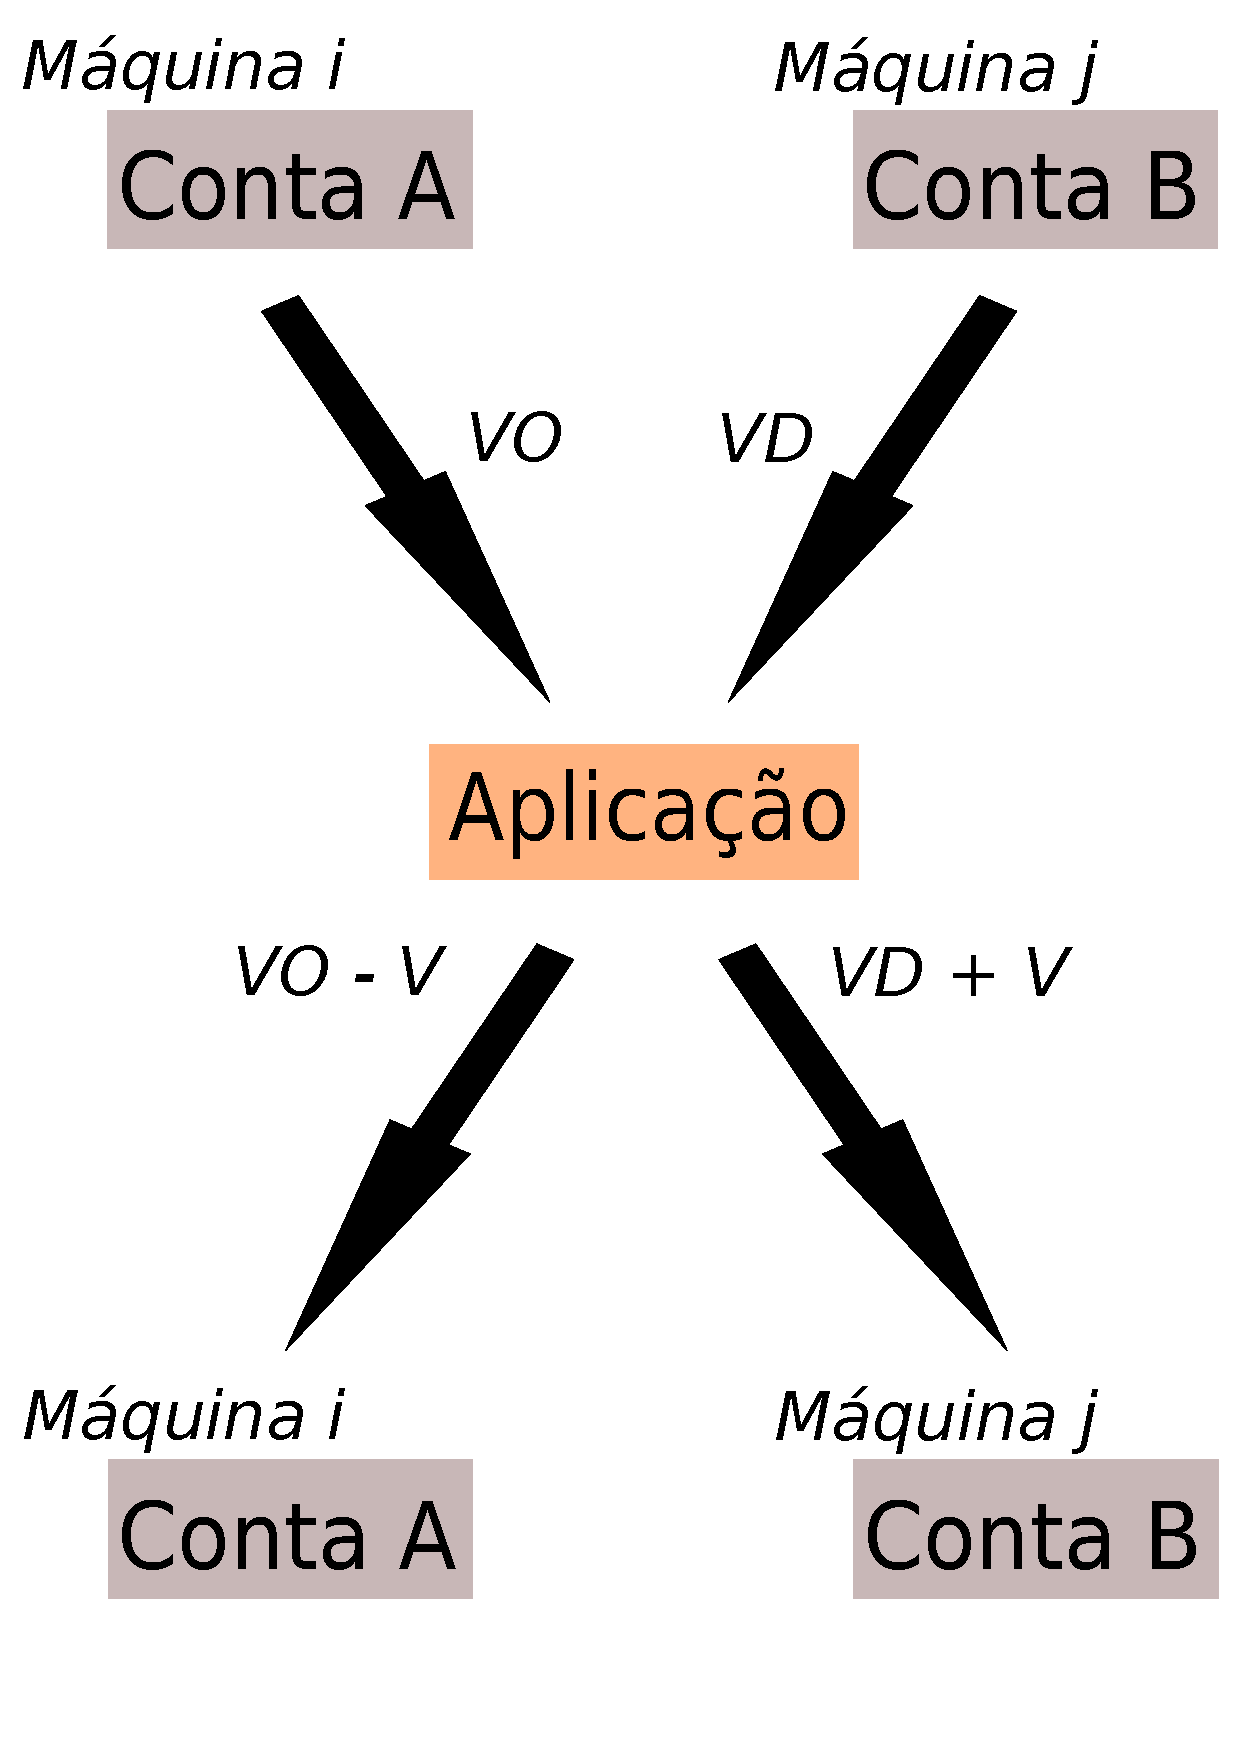
\includegraphics[width=.40\textwidth]{transacao_distribuida} 
  \caption{Esquematização de uma transação distribuída}
  \label{fig:transacao_distribuida} 
\end{figure}

A idéia desse protocolo é simples e utilizada a bastante tempo \cite{2pc}: verificar se todos os gerenciadores de recurso envolvidos em uma transação estão aptos a efetivar suas respectivas subtransações. Se estiverem, a transação será efetivada. Se algum gerenciador não puder efetivar, por qualquer motivo, a transação será abortada. Este protocolo necessita de um gerenciador que atue como o \textbf{coordenador} da transação, responsável por gerenciar a execução do protocolo e tomar a decisão sobre efetivar ou abortar a transação comunicando-se com os outros \textbf{participantes}, que executam as subtransações associadas à transação. O coordenador pode ser também um participante da transação.

Como seu nome diz, o protocolo é dividido em duas fases, ou rodadas. Na primeira fase o coordenador solicita que os participantes enviem seus votos, indicando se estão aptos a efetivar a subtransação executada. Os votos são coletados e o coordenador decide se a transação pode ser efetivada (caso todos os participantes tenham votado de acordo) ou se deve ser abortada (caso algum participante tenha votado para não efetivar a transação). Decidido o resultado da votação, o coordenador efetua a segunda fase, em que os participantes são notificados do resultado da votação. 

De forma mais detalhada, o \emph{2PC} pode ser descrito pelos algoritmos \ref{alg:2pc_coordenador}, \ref{alg:2pc_participante1} e \ref{alg:2pc_participante2}. O algoritmo \ref{alg:2pc_coordenador} descreve as ações do coordenador ao ser notificado que o protocolo deve iniciar. Os algoritmos \ref{alg:2pc_participante1} e \ref{alg:2pc_participante2} descrevem as ações executadas pelos participantes ao receberem uma solicitação de votação (primeira fase) e o resultado da votação (segunda fase), respectivamente. 

Uma estrutura de dados essencial na execução do \emph{2PC} é o registro de operações, ou \emph{log}. Ele é responsável por registrar as decisões do coordenador e dos participantes, e é gravado localmente em cada gerenciador de recursos envolvido na transação. A função $Adicionar$ representa a operação de adicionar um elemento ao final do \emph{log}. A função $Enviar(d, m)$ representa o envio de uma mensagem $m$ para um destinatário $d$, e a função $Receber(r)$ representa o recebimento de uma mensagem de um remetente $r$. Uma visualização da execução do algoritmo pode ser vista nas figuras \ref{fig:2PC_1fase} e \ref{fig:2PC_2fase}.

\begin{algorithm}
\caption{Coordenador 2PC}
\label{alg:2pc_coordenador}
\dontprintsemicolon
\Inicio{
    $Adicionar(log_c, (PREPARAR, T))$\;
    \ParaTodo{$p_i \in Participantes$}
    {
    	$Enviar(p_i, (PREPARAR, T))$\;
    }
    $d \gets EFETIVAR$\;
    \ParaTodo{$p_i \in Participantes$}
    {    
        $v \gets Receber(p_i)$\;
        \Se{$v = ABORTAR$}
        {
            $d \gets ABORTAR$\;
        }
    }
    $Adicionar(log_c, (d, T))$\;
    \ParaTodo{$p_i \in Participantes$}
    {
    	$Enviar(p_i, (d, T))$\;
    }
}
\end{algorithm}

\begin{algorithm}
\caption{Votação 2PC - $p_i$ recebe $(PREPARAR, T)$ de $c$}
\label{alg:2pc_participante1}
\dontprintsemicolon
\Inicio{
    $v \gets Decidir(T)$\;
    $Adicionar(log_i, (v, T))$\;
    $Enviar(c, v)$\;
}
\end{algorithm}

\begin{algorithm}
\caption{Notificação 2PC - $p_i$ recebe $(d, T)$ de $c$}
\label{alg:2pc_participante2}
\dontprintsemicolon
\Inicio{
    \eSe{$d = EFETIVAR$}
    {
        $Efetivar(T)$\;
        $Adicionar(log_i, (EFETIVAR, T))$\;
    }
    {
    	$Abortar(T)$\;
    	$Adicionar(log_i, (ABORTAR, T))$\;
    }
}
\end{algorithm}

A premissa que norteia o protocolo é que qualquer gerenciador envolvido na transação pode decidir abortá-la de forma unilateral, exigindo assim unanimidade na decisão pela efetivação da transação. As mensagens enviadas durante a execução do protocolo indicam uma decisão do remetente, e para garantir que essa decisão sobreviva a falhas no gerenciador que enviou a mensagem, os dados do \emph{log} são gravados em um meio de armazenamento estável, como um disco rígido, antes da mensagem ser enviada. A transação $T$ é considerada oficialmente efetivada (ou abortada) no momento que o registro de $(EFETIVAR, T)$ (ou $(ABORTAR, T)$) do \emph{log} do coordenador for escrito para a área de armazenamento estável da máquina. Falhas posteriores não podem mudar a decisão do coordenador registrada em seu \emph{log} e gravada em disco.

\begin{figure}
  \centering
  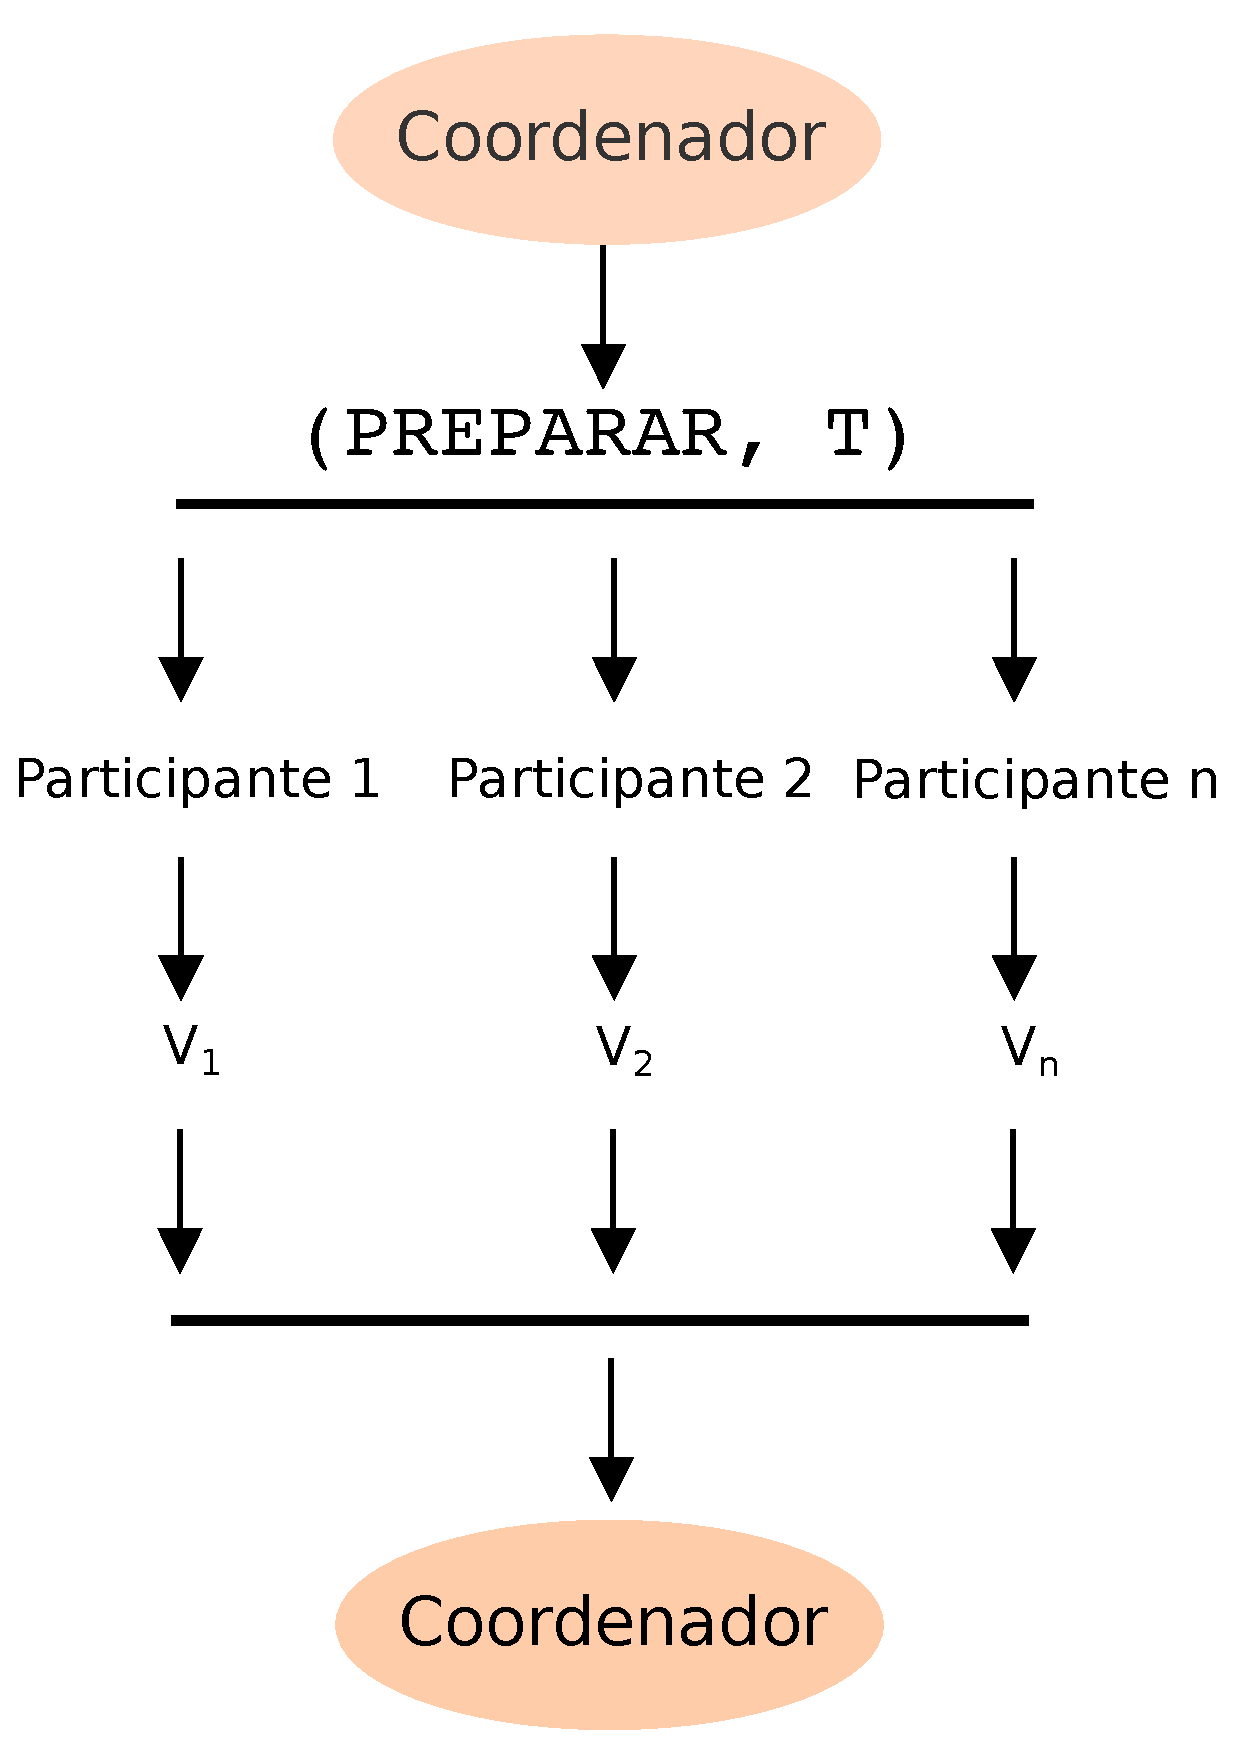
\includegraphics[width=.40\textwidth]{2PC_1fase} 
  \caption{Primeira fase 2PC - O coordenador inicia a votação e os participantes respondem com seus votos $V_i$}
  \label{fig:2PC_1fase} 
\end{figure}

\begin{figure}
  \centering
  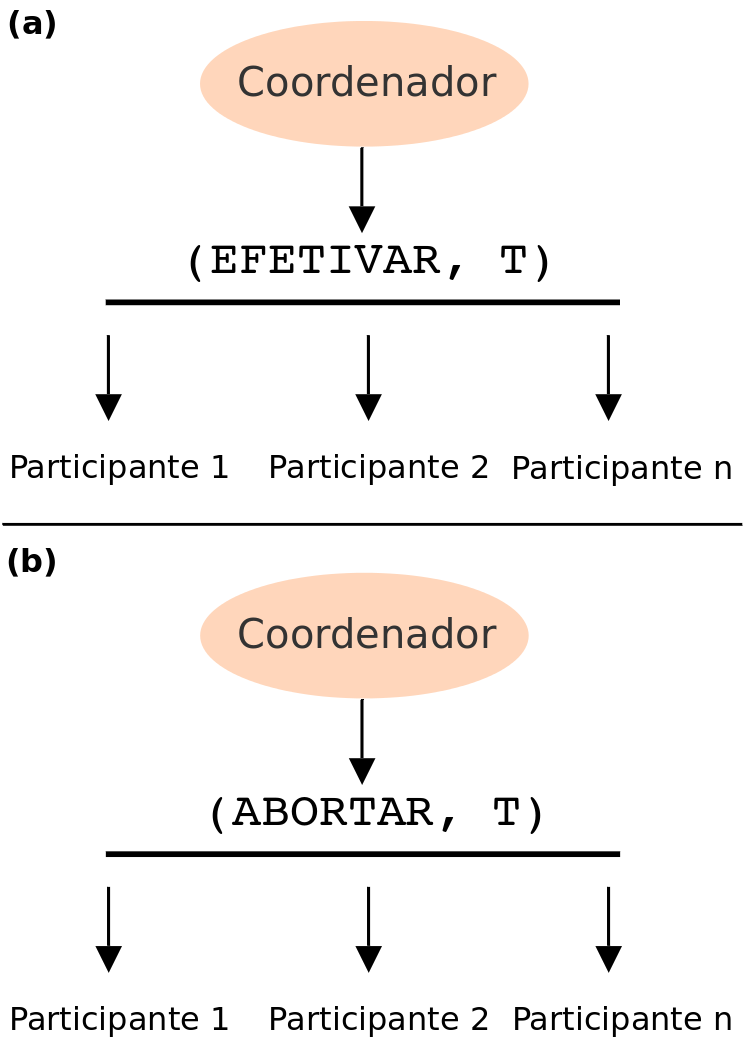
\includegraphics[width=.40\textwidth]{2PC_2fase} 
  \caption{Segunda fase 2PC- O coordenador apura os votos e notifica os participantes. Em (a) os participantes são notificados de uma efetivação. Em (b), a transação foi abortada.}
  \label{fig:2PC_2fase} 
\end{figure}

É importante notar que esse protocolo não define como as operações da transação devem ser executadas nas máquinas participantes, mas sim como a efetivação da transação deve proceder. As operações da transação devem ser executadas em cada participante antes que o protocolo de efetivação inicie. Portanto, a execução desse protocolo aumenta o número de mensagens e consequentemente o tempo e o esforço necessários para que uma transação seja executada. Algumas otimizações podem ocorrer, como no caso de transações que efetuam somente operações de leitura ou de transações que envolvam dados em somente uma máquina do sistema mas, de forma geral, a execução do \emph{2PC} é custoso \cite{gray-lamport}.

\section{Minitransações}
\label{sec:minitransacoes}
Minitransação é uma primitiva que permite que as operações de uma transação sejam executadas durante o protocolo de efetivação. Esse protocolo de efetivação é uma modificação do \emph{2PC}, e oferece um mecanismo simples para ler e alterar dados de forma condicional em um ambiente distribuído garantindo atomicidade na execução das operações \cite{sinfonia}. Dessa forma, o número de mensagens e o tempo de execução da transação são reduzidos. 

Porém, o uso das minitransações impõe certas restrições em relação ao que pode ser feito, diminuindo sua aplicabilidade. Por exemplo, o condicionamento das operações de leitura e escrita é baseado somente em comparações de igualdade, e a única forma da aplicação cliente abortar a minitransação é se essa comparação, como será detalhado. Com as minitransações originais não é possível efetuar a transferência entre contas distribuídas como no Algoritmo \ref{alg:transferencia_valores_transacao}, pois a comparação de maior ou igual ($>=$) não pode ser feita. A nossa infraestrutura irá permitir que essas outras comparações sejam feitas.

Em \ref{subsec:derivando-minitransacoes} é apresentado como o protocolo \emph{2PC} pode ser usado como ponto de partida para otimizações e para a obtenção do protocolo de minitransações e em \ref{subsec:estrutura-minitransacoes} definimos formalmente o conceito de minitransação.

\subsection{Otimização do \emph{2PC}}
\label{subsec:derivando-minitransacoes}
A decisão pela efetivação ou cancelamento de uma transação distribuída depende tanto de aspectos operacionais, relacionados ao ambiente de execução, quanto de aspectos semânticos, específicos do domínio da aplicação. A falha na execução de uma subtransação em alguma máquina do ambiente inviabiliza a efetivação da transação como um todo, e por isso o coordenador é forçado a cancelar a transação. Esse tipo de falha operacional não está ligada ao domínio da aplicação, mas sim ao ambiente em que essa aplicação está rodando e está, portanto, fora do controle do coordenador, que pode somente cancelar a transação e, opcionalmente, tentar executá-la novamente. Por outro lado, o aspecto semântico envolvido na decisão pela efetivação ou cancelamento da transação é específico de cada aplicação e depende, direta ou indiretamente, dos dados do sistema.

Considerando novamente o sistema bancário e a operação de transferência de uma determinada quantia entre uma conta de origem e de destino, a transferência só pode ocorrer se o saldo na conta de origem da transferência for maior ou igual à quantia a ser transferida. Essa checagem deve ser feita pela aplicação após a leitura da informação da máquina que armazena os dados da conta de origem, e a decisão pelo cancelamento ou não da transação fica subordinada à semântica dada aos dados do sistema. Isso exige que uma requisição de leitura seja feita e uma resposta seja enviada, para só então a aplicação decidir se vai efetivar e então, após a execução do restante da transação, iniciar a primeira fase do protocolo \emph{2PC} (votação).

Podemos ver que, do ponto de vista semântico, as operações que influenciam na decisão pela possível efetivação ou pelo cancelamento da transação são operações de leitura. As operações de escrita não influenciam nessa decisão, a não ser pelo ponto de vista operacional, ou seja, se ocorrer realmente um erro na operação de escrita. Assim, se tivermos uma transação cuja última ação não afete a decisão do coordenador sobre efetivar a transação, podemos embutir essa última ação na mensagem de votação da primeira fase do protocolo de efetivação.

O aspecto semântico da transação em relação aos dados pode ser tratado nos participantes também, e não somente no coordenador, caso o participante saiba como o coordenador irá utilizar o dado para fazer sua decisão sobre efetivar ou cancelar a transação. Se isso for possível, podemos então embutir também operações de leitura que influenciam a decisão do coordenador no protocolo de efetivação e fazer o participante adequar seu voto à maneira como o coordenador faria ao analisar o dado retornado.

As minitransações surgem no contexto em que todas as operações de uma subtransação podem ser embutidas dentro do protocolo de efetivação, utilizando somente as trocas de mensagens que ocorreriam no protocolo de efetivação, após a execução dos comandos. Para que isso possa ocorrer, as mensagens do protocolo \emph{2PC} precisam ser alteradas.

\subsection{Definição}
\label{subsec:estrutura-minitransacoes}
Uma minitransação é composta por três conjuntos: itens de comparação, itens de leitura e itens de escrita, como pode ser visto na figura \ref{fig:estrutura_minitransacao}. Todos os itens possuem uma referência a qual dado deve ser utilizado ($ID_{A...D}$), e os itens de comparação e escrita incluem também os dados ($DADO_{1...4}$) que serão comparados com ou substituirão os dados armazenados \cite{sinfonia}. 

\begin{figure}
  \centering
  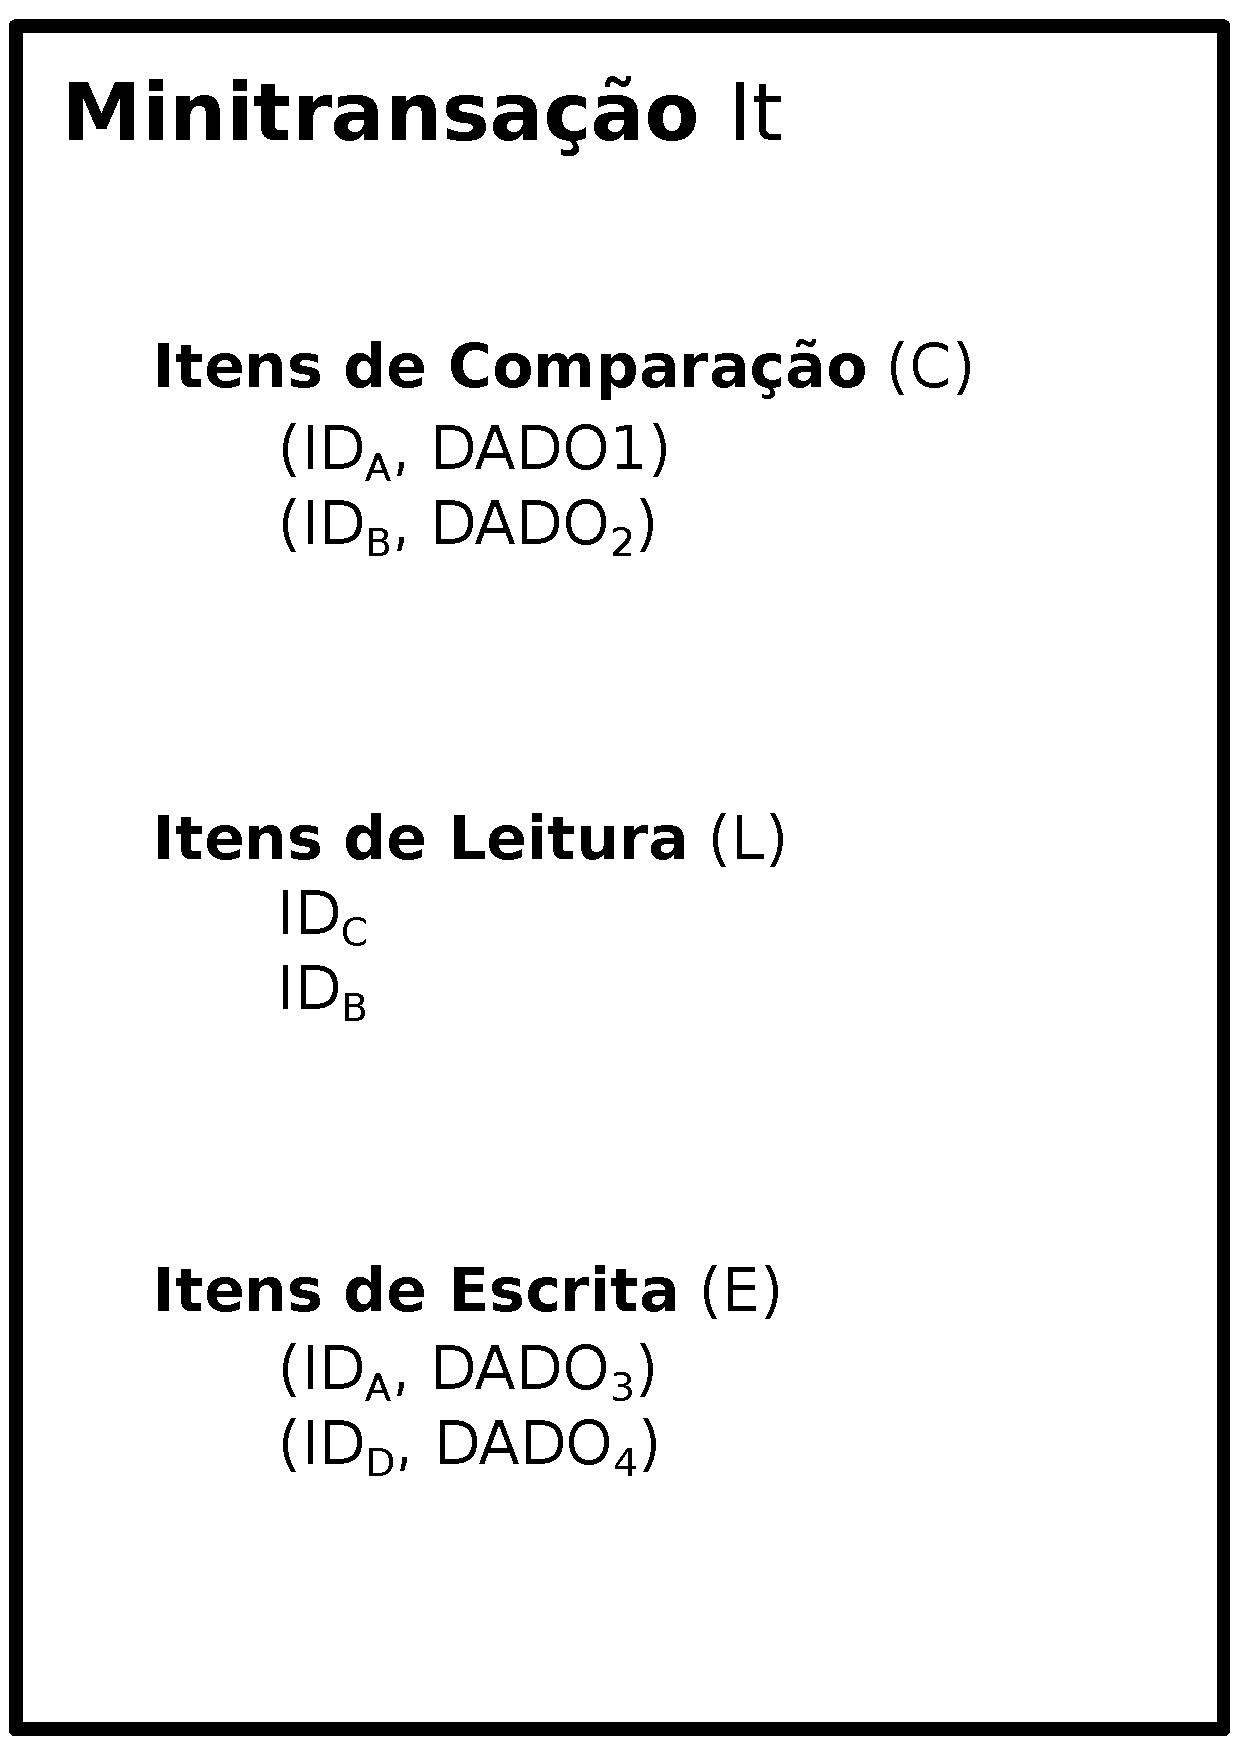
\includegraphics[width=.40\textwidth]{estrutura_minitransacao} 
  \caption{Estrutura de uma minitransação}
  \label{fig:estrutura_minitransacao} 
\end{figure}

Formalmente, uma minitransação pode ser vista como uma tupla na forma $(I, C, L, E)$. $I$ é o identificador da minitransação, gerado pelo criador da minitransação. \(C\) é o conjunto de itens de comparação, \(L\) é o conjunto de itens para leitura e \(E\) é o conjunto de itens para escrita. Os elementos de \(L\) são identificadores de dados, e o domínio de seus valores é o conjunto de identificadores armazenados na máquina participante. \(C\) e \(E\) possuem elementos que podem ser representados como tuplas no formato \((Id, Dado)\), em que \(Id\) é o identificador do dado e \(Dado\) é o valor para se comparar com o valor identificado por $Id$ ou para substituí-lo.

Sendo uma extensão do \emph{2PC}, o protocolo de minitransações possui também um coordenador responsável por iniciar e gerenciar a execução do protocolo entre os participantes da transação. O protocolo de minitransações é composto também por duas fases, mas agora a primeira fase passa a ser uma fase de execução, em que as minitransações são executadas em cada participante e seus votos são enviados para o coordenador. O coordenador coleta os votos de todos os participantes e, como no protocolo original, irá decidir por efetivar a transação somente se os votos forem unânimes. Na segunda fase os participantes são notificados da decisão do coordenador e devem atuar de acordo, efetivando as operações da minitransação ou desfazendo as seus ações.

Uma função especial, $Id[X]$, representa o conjunto formado pelo elemento $Id$ de todas as tuplas no formato $(Id, Dado)$ do conjunto $X$. Essa função permite obter o conjunto $D$ de todos os identificadores utilizados pela minitransação: $D \gets L \cup Id[C] \cup Id[E]$. Cada elemento de $D$ fica sob responsabilidade de um participante $p$ específico da minitransação, e $\forall d \in D$ o participante responsável pelo identificador $d$ é definido por $Participante(d)$, uma função que indica que $p$ é a possível localização de $d$ entre os participantes, uma vez que o identificador $d$ pode ainda não ter sido inserido em $p$.

O conjunto $Participantes$ é formado por todos os participantes da minitransação. Cada participante $P_j \in Participantes$ possui um conjunto $K_j$ de identificadores sob sua responsabilidade, e para cada participante o coordenador constrói uma nova minitransação \(M_j = (I_t, C_j, L_j, E_j)\) tal que:

\begin{itemize}
    \item $I_t \gets IdentificadorUnico(I)$
    \item $\forall i_l \in L_j, i_l \in K_j$;
    \item $\forall i_c \in Id[C_j], i_c \in K_j$; e
    \item $Id[E_j] \supseteq K_j$
\end{itemize}

O identificador $I_t$ é unicamente definido e associado ao identificador $I$ por meio da função $IdentificadorUnico$. Como o identificador $I$ é fornecido pela aplicação cliente, nada garante que ele seja único, e por isso utilizamos $IdentificadorUnico$ para criar um novo identificador globalmente único associado à $I$. Os identificadores de $E_j$ são tratados como um superconjunto de $K_j$ pois a operação de escrita pode inserir novos dados no sistema, e não somente alterar dados que já existem.

Cada $M_j$ é enviada ao respectivo $P_j$ pelo coordenador, que irá esperar pela execução e resposta de cada participante. Ao receber uma minitransação, cada participante irá tentar ler os dados identificados por $Id[C_j]$ e compará-los (comparação de igualdade) com os respectivos $Dado[C_j]$. Caso a comparação não seja bem sucedida, esse participante nem tentará ler ou modificar os dados em $L_j$ e $E_j$, e responderá para o coordenador com um voto $ABORTAR$. A Figura \ref{fig:minitransacao_1fase} ilustra essa primeira fase, que combina a primeira fase do \emph{2PC} com a execução das operações da transação.

\begin{figure}
  \centering
  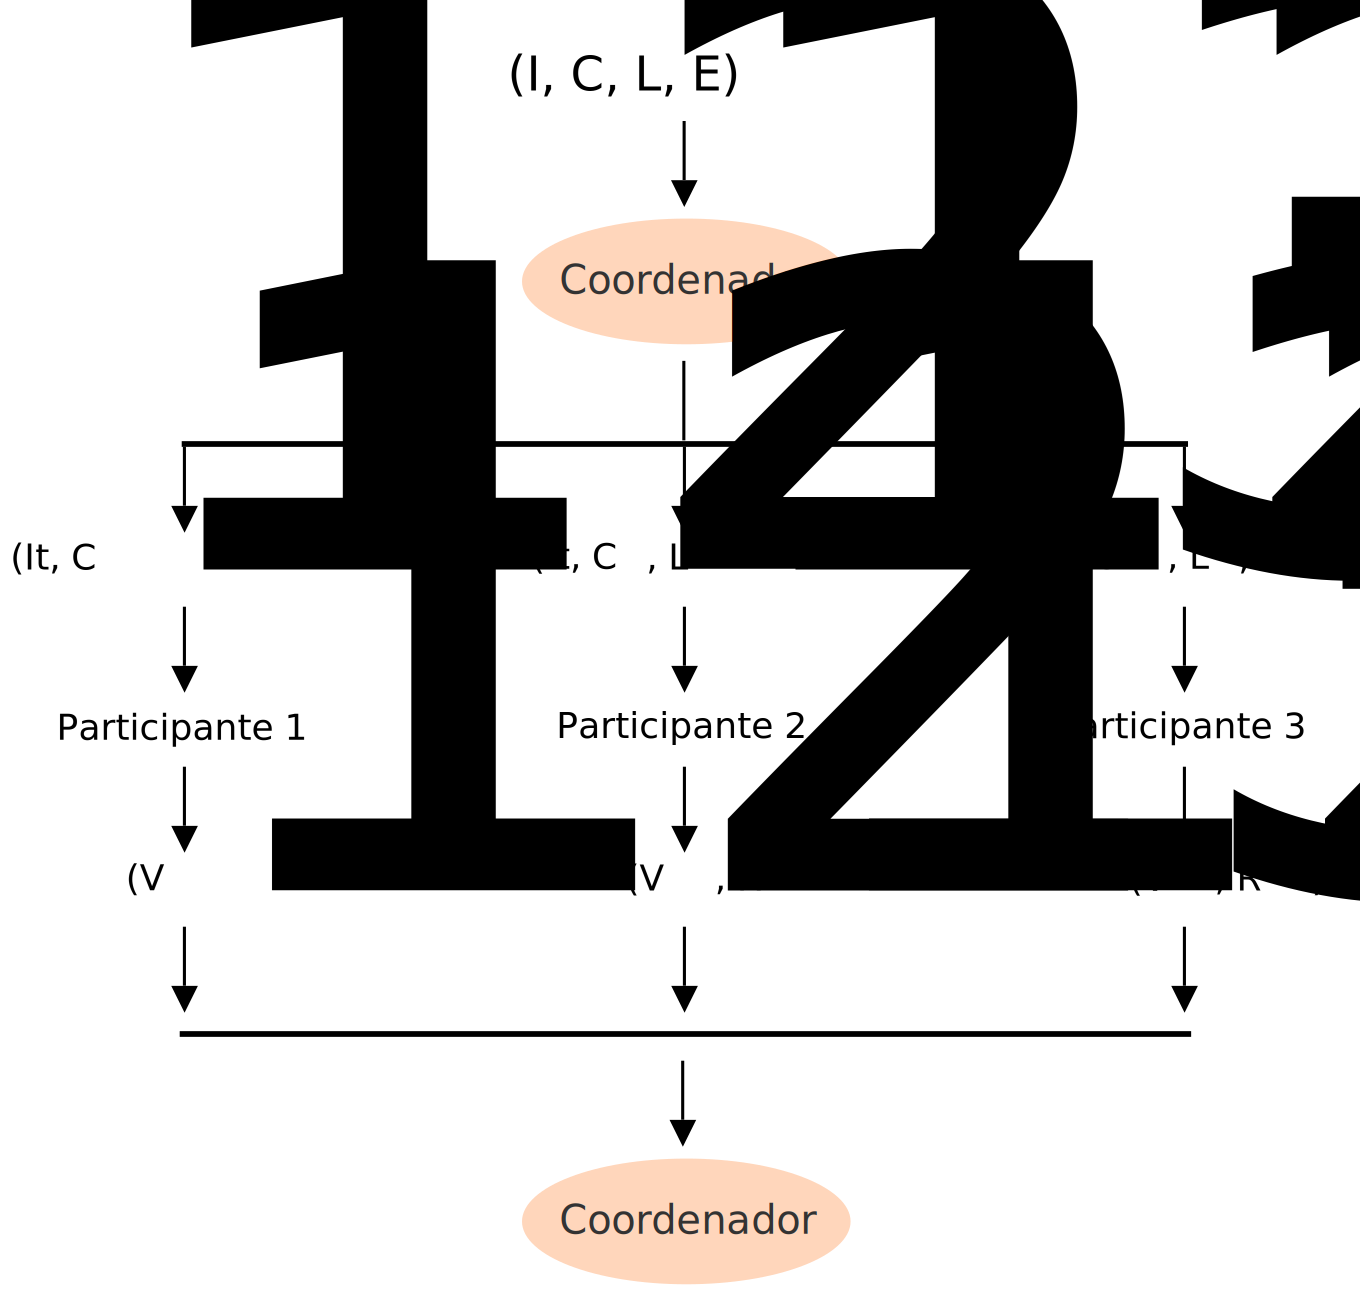
\includegraphics[width=.80\textwidth]{minitransacao_1fase} 
  \caption{Fase de execução de uma minitransação}
  \label{fig:minitransacao_1fase} 
\end{figure}

Se a comparação for bem sucedida para todos os elementos de $Id[C_j]$, então o participante irá ler os dados identificados por $L_J$ e agrupá-los no conjunto de resposta $R_j$. Os dados $Dado[E_j]$ identificados por $Id[E_j]$ serão inseridos no conjunto de dados ou irão alterar algum dado já existente. Na verdade, a operação de inserir ou alterar um dado é registrada no \emph{log} do participante. O participante envia então um voto $EFETIVAR$ para o coordenador, junto com o conjunto $R_j$. 

Ao coletar todas as respostas, o coordenador irá apurar os votos de cada participante. Para cada resposta $EFETIVAR$ o coordenador agrega os respectivos $R_j$ em um conjunto de respostas $R$. Se uma das respostas for $ABORTAR$, a transação precisa ser abortada, notificando os participantes do cancelamento, e a aplicação cliente precisa ser notificada desse erro. Se não houve nenhum voto $ABORTAR$, o coordenador decide então por efetivar a transação, enviando o conjunto $R$ para a aplicação cliente e notificando os participantes da efetivação. Os dois casos possíveis para a segunda fase descritos podem ser vistos na Figura \ref{fig:minitransacao_2fase}.

\begin{figure}
  \centering
  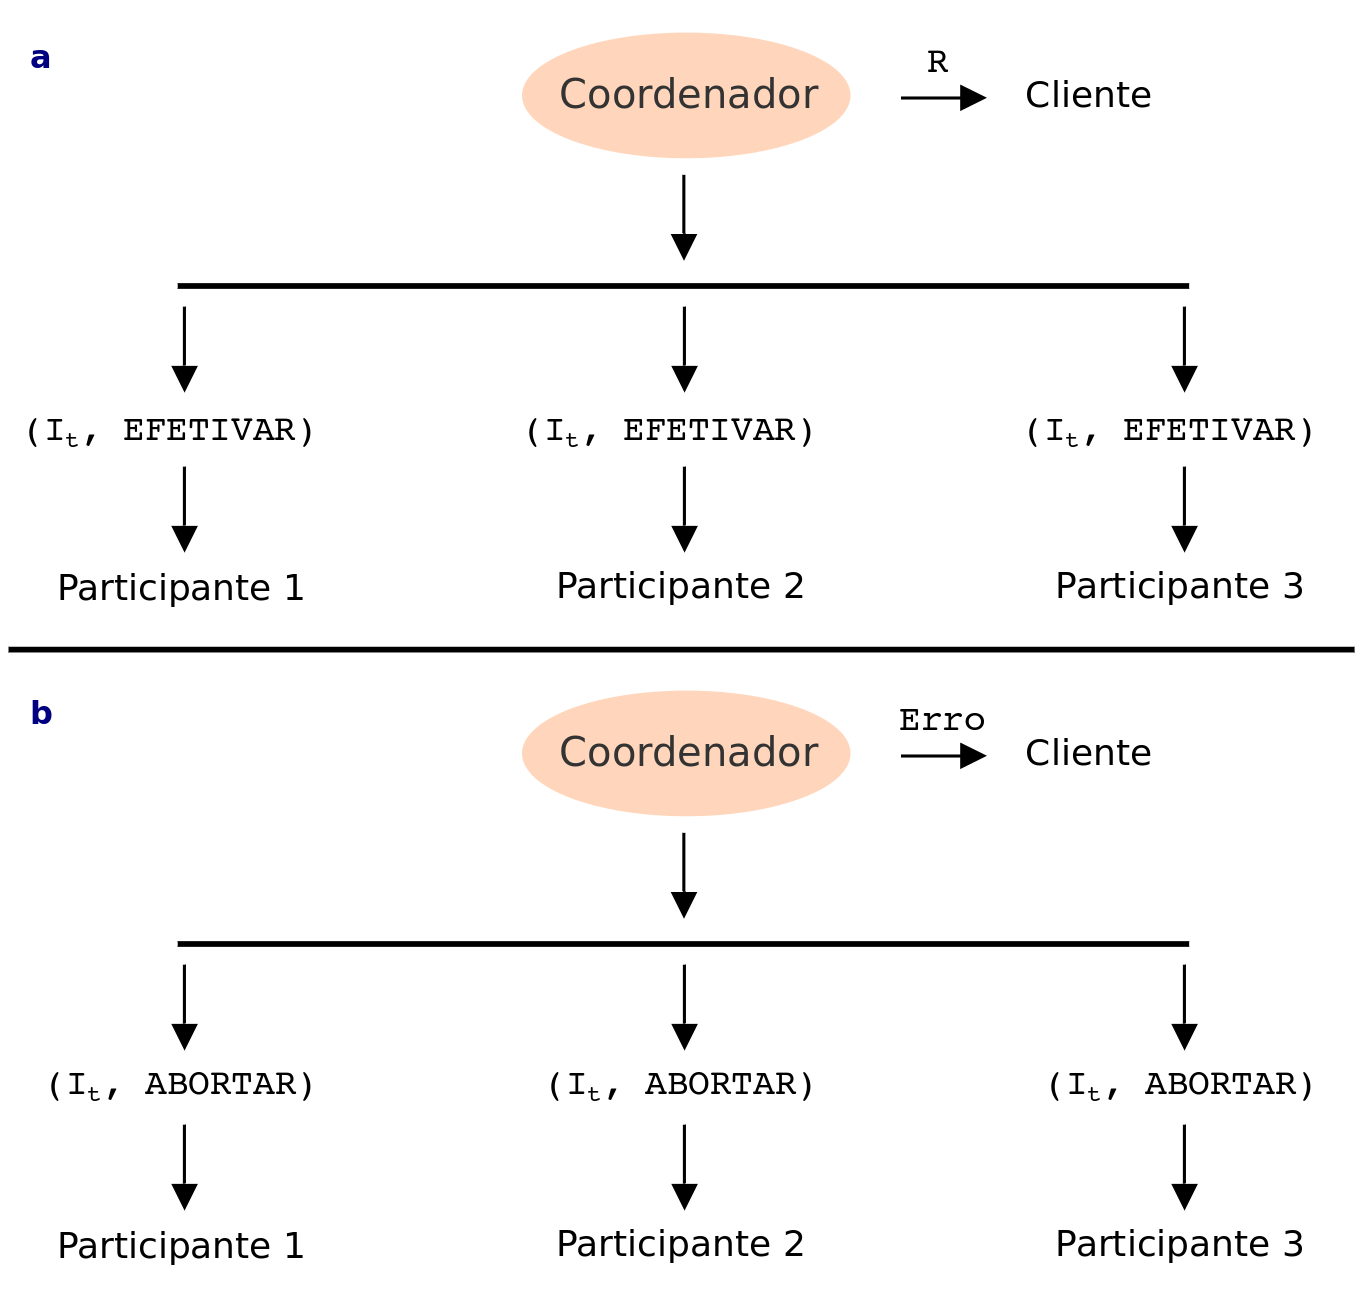
\includegraphics[width=.80\textwidth]{minitransacao_2fase} 
  \caption{Fase de notificação de uma minitransação}
  \label{fig:minitransacao_2fase} 
\end{figure}

Quando os participantes são notificados do cancelamento da minitransação, as operações de escrita da minitransação presentes no \emph{log} do participante não serão efetuadas, deixando os dados inalterados, e será registrado no \emph{log} que a minitransação foi abortada. Se a notificação for de efetivação, as operações de escrita do \emph{log} serão efetuadas, alterando dados existentes ou inserindo novos dados no participante, e será registrado no \emph{log} que a minitransação foi efetivada. O \emph{log} será gravado em disco e a minitransação será considerada oficialmente efetivada ou abortada no momento que esse registro do \emph{log} estiver gravado em disco.

\chapter{A infraestrutura}
\label{chap:implementacao}
Neste capítulo apresentamos uma visão detalhada da infraestrutura desenvolvida. A arquitetura e a interface de acesso serão discutidas na Seção \ref{sec:arquitetura}. A Seção \ref{sec:algoritmos} descreve as estruturas de dados e algoritmos utilizados para implementar a execução das minitransações. Na Seção \ref{sec:trabalhos_relacionados} são apresentados os trabalhos que compartilham características de nossa infraestrutura, assim como suas diferenças em relação à nossa infraestrutura. 

No trabalho descrito em \cite{sinfonia} as minitransações podem ser compostas por apenas três tipos de operações: Leitura, Escrita e Comparação por igualdade. Essa estrutura permite que uma grande quantidade de transações possam ser descritas como uma minitransação, mas exclui uma série de outros tipos de transação. Por esse motivo, a nossa infraestrutura estenderá o conceito original de minitransação e permitirá que operações sejam definidas e utilizadas pelos usuários, de maneira semelhante à utilização de um procedimento armazenado (\emph{stored procedure}) de um banco de dados convencional. Esses comandos serão chamados daqui em diante de Comandos de Extensão ou Extensões.

Assim, esperamos flexibilizar a utilização e aumentar o número de cenários em que a infraestrutura pode ser utilizada. Portanto, a estrutura das minitransações descrita neste capítulo difere um pouco da estrutura descrita em \ref{subsec:estrutura-minitransacoes}. As operações de leitura e escrita originais serão mantidas pois possuem uma semântica diferenciada. A operação de comparação original (comparação por igualdade) será implementada como uma extensão em nossa infraestrutura.

\section{Arquitetura e interface de acesso}
\label{sec:arquitetura}
A infraestrutura desenvolvida neste trabalho é um sistema composto por dois tipos de componentes de maior importância: execução e acesso. O componente de execução é responsável por prover acesso aos dados através da execução das operações especificadas nas minitransações, e é chamado de \emph{nó de memória}. O coordenador é o ponto de comunicação entre a aplicação e a infraestrutura, atuando como o coordenador das transações e isolando a aplicação cliente dos detalhes sobre a distribuição dos dados entre os nós de memória e será chamado \emph{coordenador}. O terceiro componente é um componente de gerenciamento, utilizado para operar o sistema manualmente, chamado \emph{gerenciador}.

Os nós de memória formam o núcleo da infraestrutura e serão implementados de tal forma que não haverá nenhum compartilhamento de informação entre eles, constituindo uma arquitetura não compartilhada (\emph{shared nothing architecture} \cite{shared_nothing}) e permitindo que a infraestrutura possa escalar para acomodar uma grande quantidade de dados e atender um número crescente de usuários.

A figura \ref{fig:overview_arquitetura} ilustra a relação entre os componentes do sistema. As aplicações cliente acessam somente os coordenadores. Nesse exemplo há quatro nós de memória (\emph{Nó 1} até \emph{Nó 4}) que armazenam os dados e executam as minitransações. O gerenciador é um componente secundário, que permite a execução de procedimentos de gerenciamento sobre os nós de memória, como recuperação de falhas ou a criação dos comandos de extensão.

\begin{figure}
  \centering
  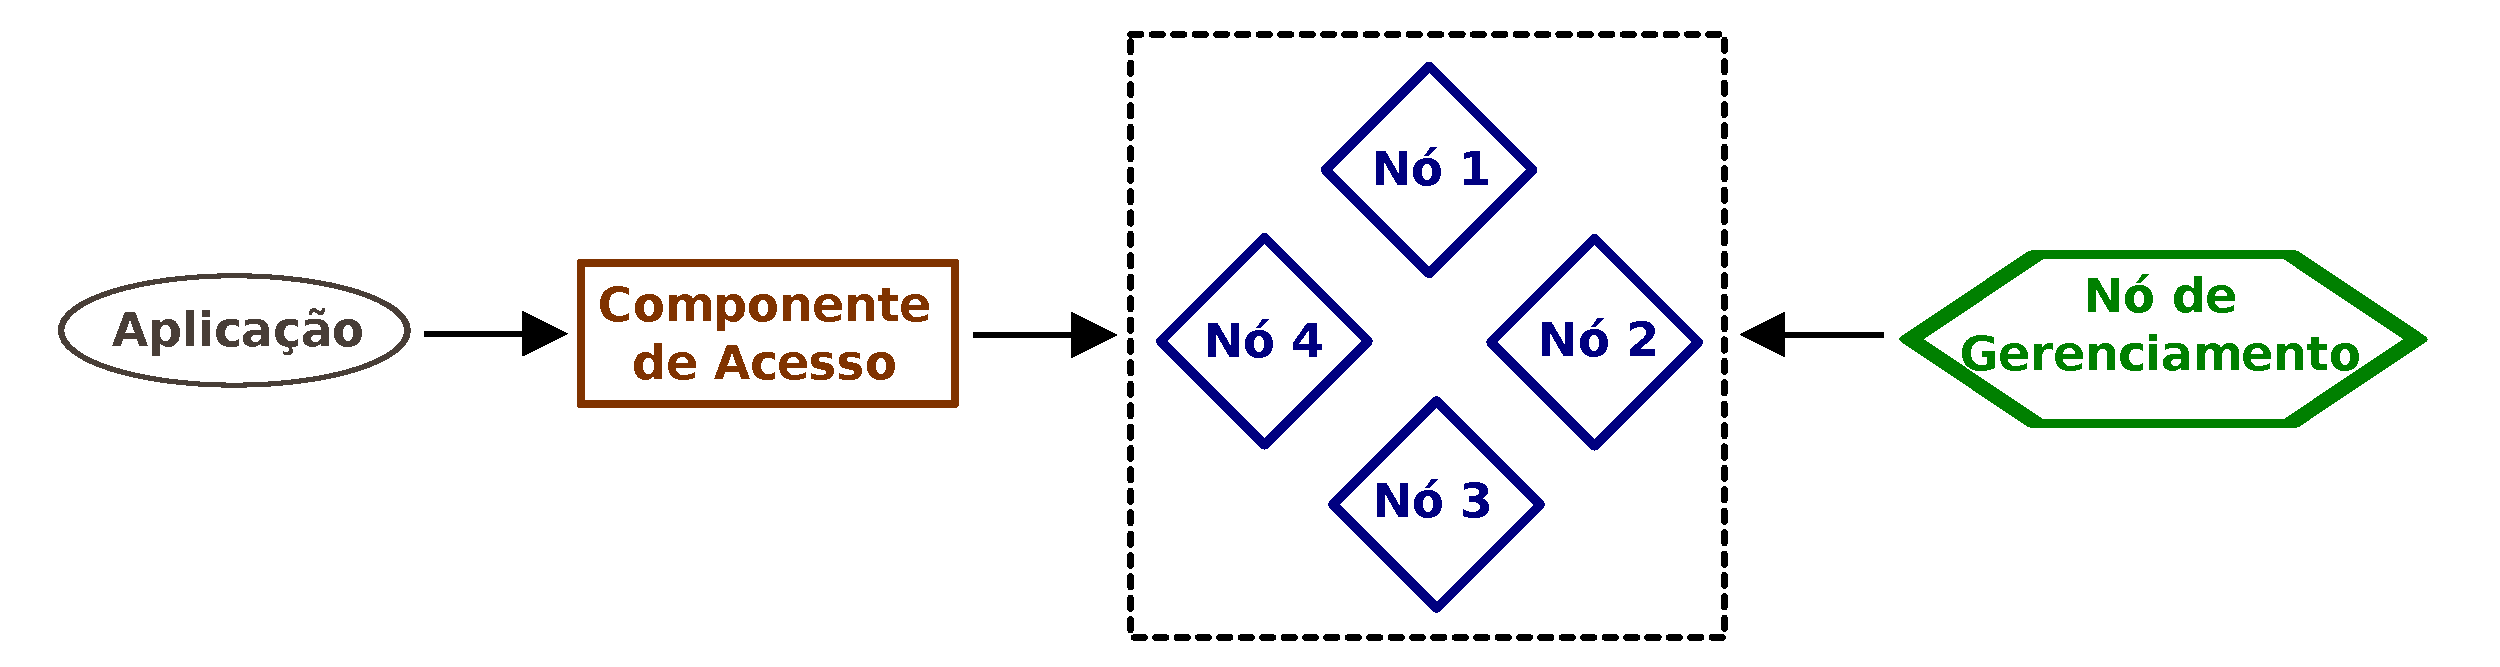
\includegraphics[width=.90\textwidth]{overview_arquitetura} 
  \caption{Visão geral da arquitetura da infraestrutura}
  \label{fig:overview_arquitetura} 
\end{figure}

A interface de acesso oferecida aos clientes da infraestrutura é a de uma tabela associativa chave-valor: os nós de memória armazenam uma sequência de bytes (valor) nomeados por uma outra sequência de bytes (chave). Cada chave é única e o número de bytes utilizados para armazenar o valor é, teoricamente, ilimitado. Os coordenadores são responsáveis por efetuar o mapeamento entre as chaves e os nós de memória que armazenam esses dados, utilizando uma função de espalhamento consistente (\emph{consistent hashing} \cite{consistent_hashing}) aplicada à chave acessada. Como pode ser visto na Figura \ref{fig:funcao_espalhamento}, o coordenador irá aplicar uma função de espalhamento consistente \textbf{$F$} à $Chave$, resultando em um número que indica que $Valor$ deve ser armazenado no nó de memória 2. 

\begin{figure}
  \centering
  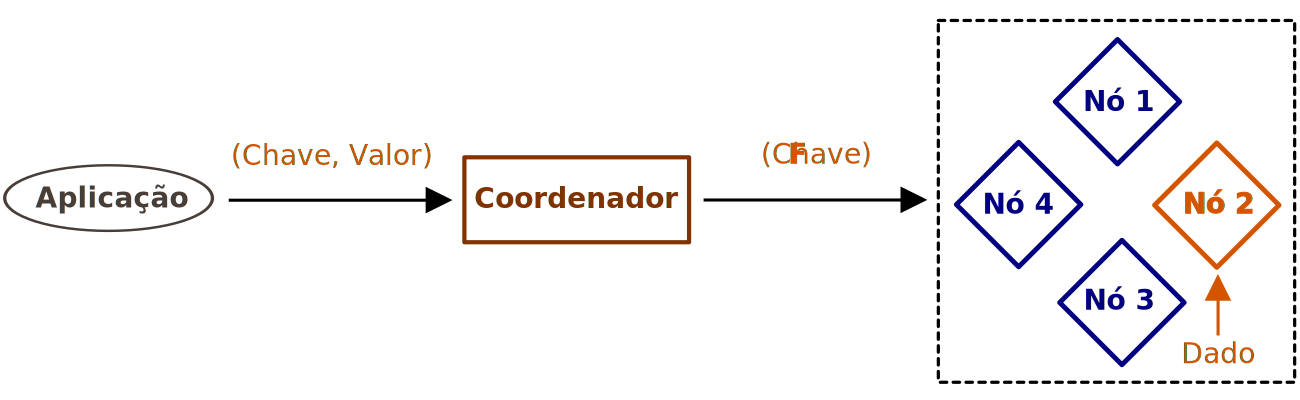
\includegraphics[width=.80\textwidth]{funcao_espalhamento} 
  \caption{Mapeamento entre a chave e o nó de memória responsável por seu armazenamento}
  \label{fig:funcao_espalhamento} 
\end{figure}

As aplicações se comunicam com os coordenadores por meio de um protocolo simples da camada de aplicação da pilha TCP/IP. Esse protocolo é textual, como o protocolo HTTP (\emph{Hypertext Transmission Protocol}), utilizando o protocolo TCP para o transporte de dados. 

\begin{figure}
  \centering
  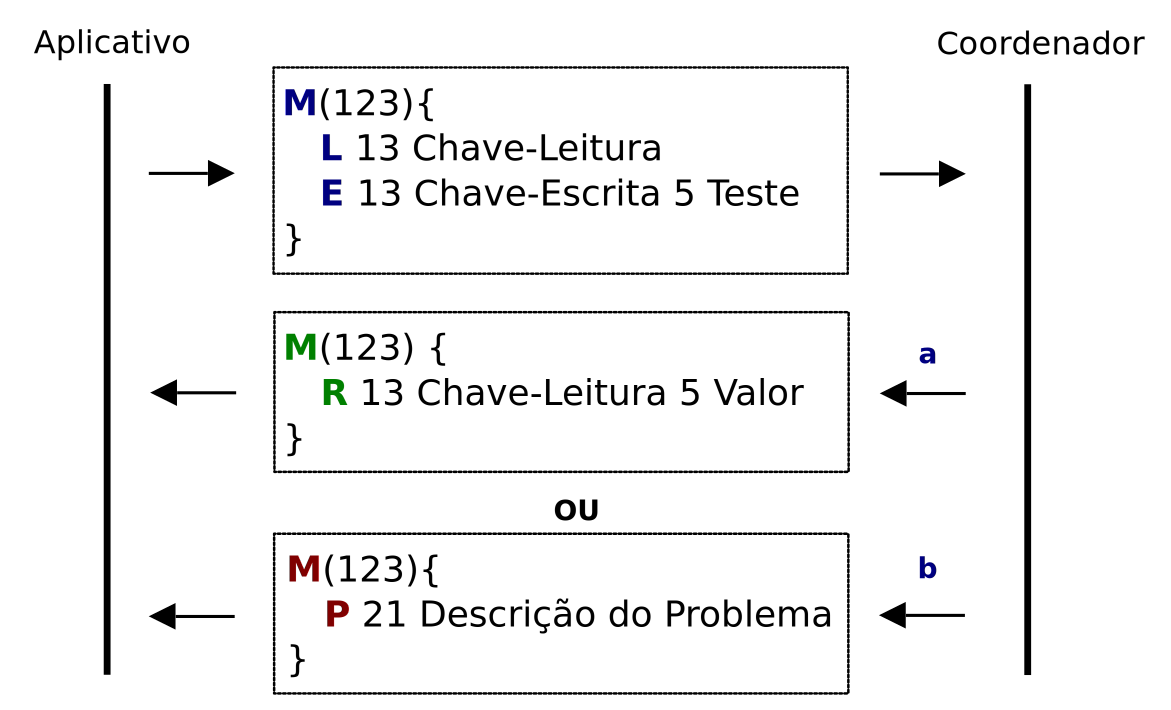
\includegraphics[width=.80\textwidth]{protocolo} 
  \caption{Exemplo de execução de uma minitransação por meio do protocolo textual utilizado entre as aplicações e o coordenador com os dois possíveis resultados: (a) A transação é bem sucedida e foi efetivada e (b) A transação fo cancelada}
  \label{fig:protocolo} 
\end{figure}

Os comandos do protocolo são separados em linhas e são compostos por uma letra, que indica a ação desse comando, e um conjunto de parâmetros, chamados campos, que fornecem informações para a execução da ação. Os comandos que iniciam uma minitransação e que contém a resposta da execução dessa minitransação podem ser compostos por subcomandos, e por isso são utilizadas chaves (\{\}) para delimitar o seu escopo. Os campos de cada comando são separados por um caracter de espaço em branco (`` ''). Os comandos disponíveis para utilização estão listados a seguir:

\begin{itemize}
    \item \textbf{M}(\textit{Identificador}): indica a criação ou execução de uma minitransação com identificador \textit{Identificador}. É composto por subcomandos, como leitura ou escrita, e o seu escopo é delimitado por chaves (\{ e \}).

    \item \textbf{L} \textit{TamanhoChave} \textit{Chave}: indica a leitura dos bytes associados à chave \textit{Chave}. \textit{TamanhoChave} indica o número de bytes de \textit{Chave}.

    \item \textbf{E} \textit{TamanhoChave} \textit{Chave} \textit{TamanhoDado} \textit{Dado}: indica a escrita de \textit{Dado}, cujo número de bytes é \textit{TamanhoDado}, no valor associado à \textit{Chave}.

    \item \textbf{C} \textit{IdentificadorComando} \textit{TamanhoChave} \textit{Chave} \textit{TamanhoParâmetro1} \textit{Parâmetro1} \textit{TamanhoParâmetro2} \textit{Parâmetro2}, ...: indica a execução de um comando de extensão identificado por \textit{IdentificadorComando} sobre a chave \textit{Chave}. Os parâmetros adicionais são repassados ao comando, que vai interpretá-los apropriadamente. Como \textit{IdentificadorComando} é composto por 4 bytes, a infraestrutura pode conter até $2^{32}$ comandos de extensão. Estes comandos não tem a permissão de escrita em nenhum dado do sistema.

    \item \textbf{R} \textit{TamanhoChave} \textit{Chave} \textit{TamanhoDado} \textit{Dado}: indica a resposta de um comando de leitura dos bytes associados à \textit{Chave}.

    \item \textbf{P} \textit{TamanhoDescrição} \textit{Descrição}: indica que ocorreu um erro e que a minitransação não pode ser executada. \textit{Descrição} contém informações sobre o erro ocorrido.
\end{itemize}

A Figura \ref{fig:protocolo} ilustra a interação entre a aplicação e o coordenador para a execução de uma minitransação cujo identificador é \textit{123} (\textbf{M}(\textit{123})). Essa minitransação possui dois subcomandos: a leitura da chave ``Chave-Leitura'' (\textbf{L} \textit{13 Chave-Leitura}) e a escrita de ``Teste'' na chave ``Chave-Escrita'' (\textbf{E} \textit{13 Chave-Escrita 5 Teste}). Como as chaves são formadas por uma sequência de bytes arbitrária, é necessário que seja especificado quantos bytes fazem parte da chave. Pelo mesmo motivo é necessário também informar o número de bytes do valor do campo ``Dado''.

No exemplo podemos ver os dois cenários de resposta. Em \textbf{a}, a execução da minitransação é bem sucedida e o participante retorna um subcomando de resposta de leitura (\textbf{R} \textit{13 Chave-Leitura 5 Valor}). 
No cenário \textbf{b}, a execução não foi bem sucedida e o coordenador notifica a aplicação através do comando \textbf{P}, descrevendo o erro ocorrido.

O protocolo de execução de minitransações usado internamente entre os coordenadores e os nós de memória é composto por um superconjunto dos comandos do protocolo descrito anteriormente. Os comandos adicionais são:

\begin{itemize}
    \item \textbf{S}: Esse comando sem parâmetros indica que a minitransação foi executada com sucesso no nó de memória, e essa minitransação está pronta para ser efetivada.

    \item \textbf{N} \textit{TamanhoDescrição} \textit{Descrição}: Esse comando indica que a execução da minitransação não foi bem sucedida e a transação precisa ser cancelada. O parâmetro \textit{Descrição} contém informações relevantes sobre o problema encontrado ao executar a minitransação.

    \item \textbf{F}: É o comando enviado pelo coordenador para os participantes para informar que a transação foi bem sucedida em todos os nós e que deve ser efetivada.

    \item \textbf{A}: Indica que a transação foi abortada e que os nós de memória devem descartar as possíveis alterações executadas pela minitransação.
\end{itemize}

Os dois primeiros comandos, \textbf{S} e \textbf{N}, são as possíveis respostas dos nós de memória à fase de execução do protocolo indicando, respectivamente, que a transação pode ou não pode ser efetivada. No caso negativo, o nó de memória irá informar no parâmetro \textit{Descrição} o motivo. Os comandos \textbf{F} e \textbf{A} são enviados do coordenador para os nós de memória para indicar que a transação foi ou não efetivada, ficando a cargo dos nós de memória os procedimentos para efetivar ou cancelar as alterações efetuadas pelas minitransações.

\section{Algoritmos e estruturas de dados}
\label{sec:algoritmos}
Iremos considerar que os dados da infraestrutura estão distribuídos em $n$ nós de memória $P_1, P_2, \dotsc, P_n$. Cada $P_i$ armazena um conjunto de informações $D_i$. O conjunto de dados $D = \bigcup_{i=1}^n D_i$ representa então o estado do sistema, e os elementos de cada $D_i$ são disjuntos. Existem duas estruturas de dados principais utilizadas pelos nós de memória e mais duas estruturas adicionais para o controle de concorrência e de falhas:

\begin{itemize}

    \item \textbf{Tabela de dados}: Cada conjunto \(D_i\) é representado por uma tabela associativa, que pode ser vista como uma função que associa um identificador a um valor, representados respectivamente por \(Id(X)\) e \(Dado(X)\), onde \(X \in D_i\). Essa tabela suporta as seguintes operações:

    \begin{enumerate}
        \item $Ler(Id(X))$, que retorna $Dado(X)$ ou um valor especial ($NULO$) caso $X \notin D_i$

        \item $Escrever(Id(X), V)$, que atribui a $Dado(X)$ o valor $V$ caso $X \in D_i$ ou que insere $X$ em $D_i$ ($D_i \gets D_i \cup \{X\}$) caso contrário. 
    \end{enumerate}
 
    \item \textbf{Registro de operações} (\emph{log}): É uma lista ordenada de operações de escrita sobre os dados. Os elementos dessa lista estão no formato $(Id(X),$ $Dado(X),$ $Dado'(X))$ onde $Id(X)$ e $Dado(X)$ são o identificador e o valor do elemento $X$ armazenado na tabela de dados, e $Dado'(X)$ é o novo valor do elemento $X$ que deve ser associado a $Dado(X)$ caso a minitransação $I_t$ seja efetivada. Essa estrutura permite que as operações de transações efetivadas sejam aplicadas corretamente e permite que o sistema se recupere de falhas. As seguintes operações são suportadas pelo \emph{log}:

        \begin{enumerate}
            \item $Adicionar(l, t, o)$, que adiciona uma operação $o$ da transação $t$ ao final da lista de operações identificada por $l$.

            \item $Selecionar(l, t)$, retorna uma lista de operações registradas em $l$ referentes à minitransação $t$.

            \item $Gravar(l)$, que força que o registro de operações identificado por $l$ seja gravado em alguma forma de armazenamento persistente, como um disco rígido.
        \end{enumerate}

    \item \textbf{Tabela de minitransações}: É um conjunto que registra a situação de uma determinada minitransação identificada por $I_t$. As possíveis situações de uma minitransação podem ser $AGUARDANDO$, $EFETIVADA$ ou $CANCELADA$.

    \item \textbf{Tabela de travas}: Associa a uma chave $c$ dois possíveis valores, chamados travas: $LEITURA$ e $ESCRITA$. A função $Travar(I_t, L, E)$ tenta associar aos elementos de $L$ a trava $LEITURA$ e aos elementos de $E$ a trava $ESCRITA$, retornando $TRAVOU$ caso seja possível, ou $FALHOU$ caso contrário. A função $Liberar(I_t)$ retira todas as travas associadas à transação $I_t$.
\end{itemize}

Um exemplo das operações sobre as estruturas principais e a relação entre elas pode ser visto na figura \ref{fig:estruturas}. Nessa figura, são executadas duas operações: uma leitura de ``Chave 1'', resultando em ``Dado 1'', e uma escrita em ``Chave N'', resultando na alteração do valor associado à essa chave para ``ABC''. Antes que essas duas operações possam ocorrer, são obtidas duas travas---uma de leitura para a chave ``Chave 1'' e uma de escrita para a chave ``Chave N''. O registro $(I_T, Chave\ N, Dado\ N, ABC)$ é adicionado ao \emph{log} de operações, e o elemento $\{I_t, AGUARDANDO\}$ é incluído na tabela de minitransações.

\begin{figure}
  \centering
  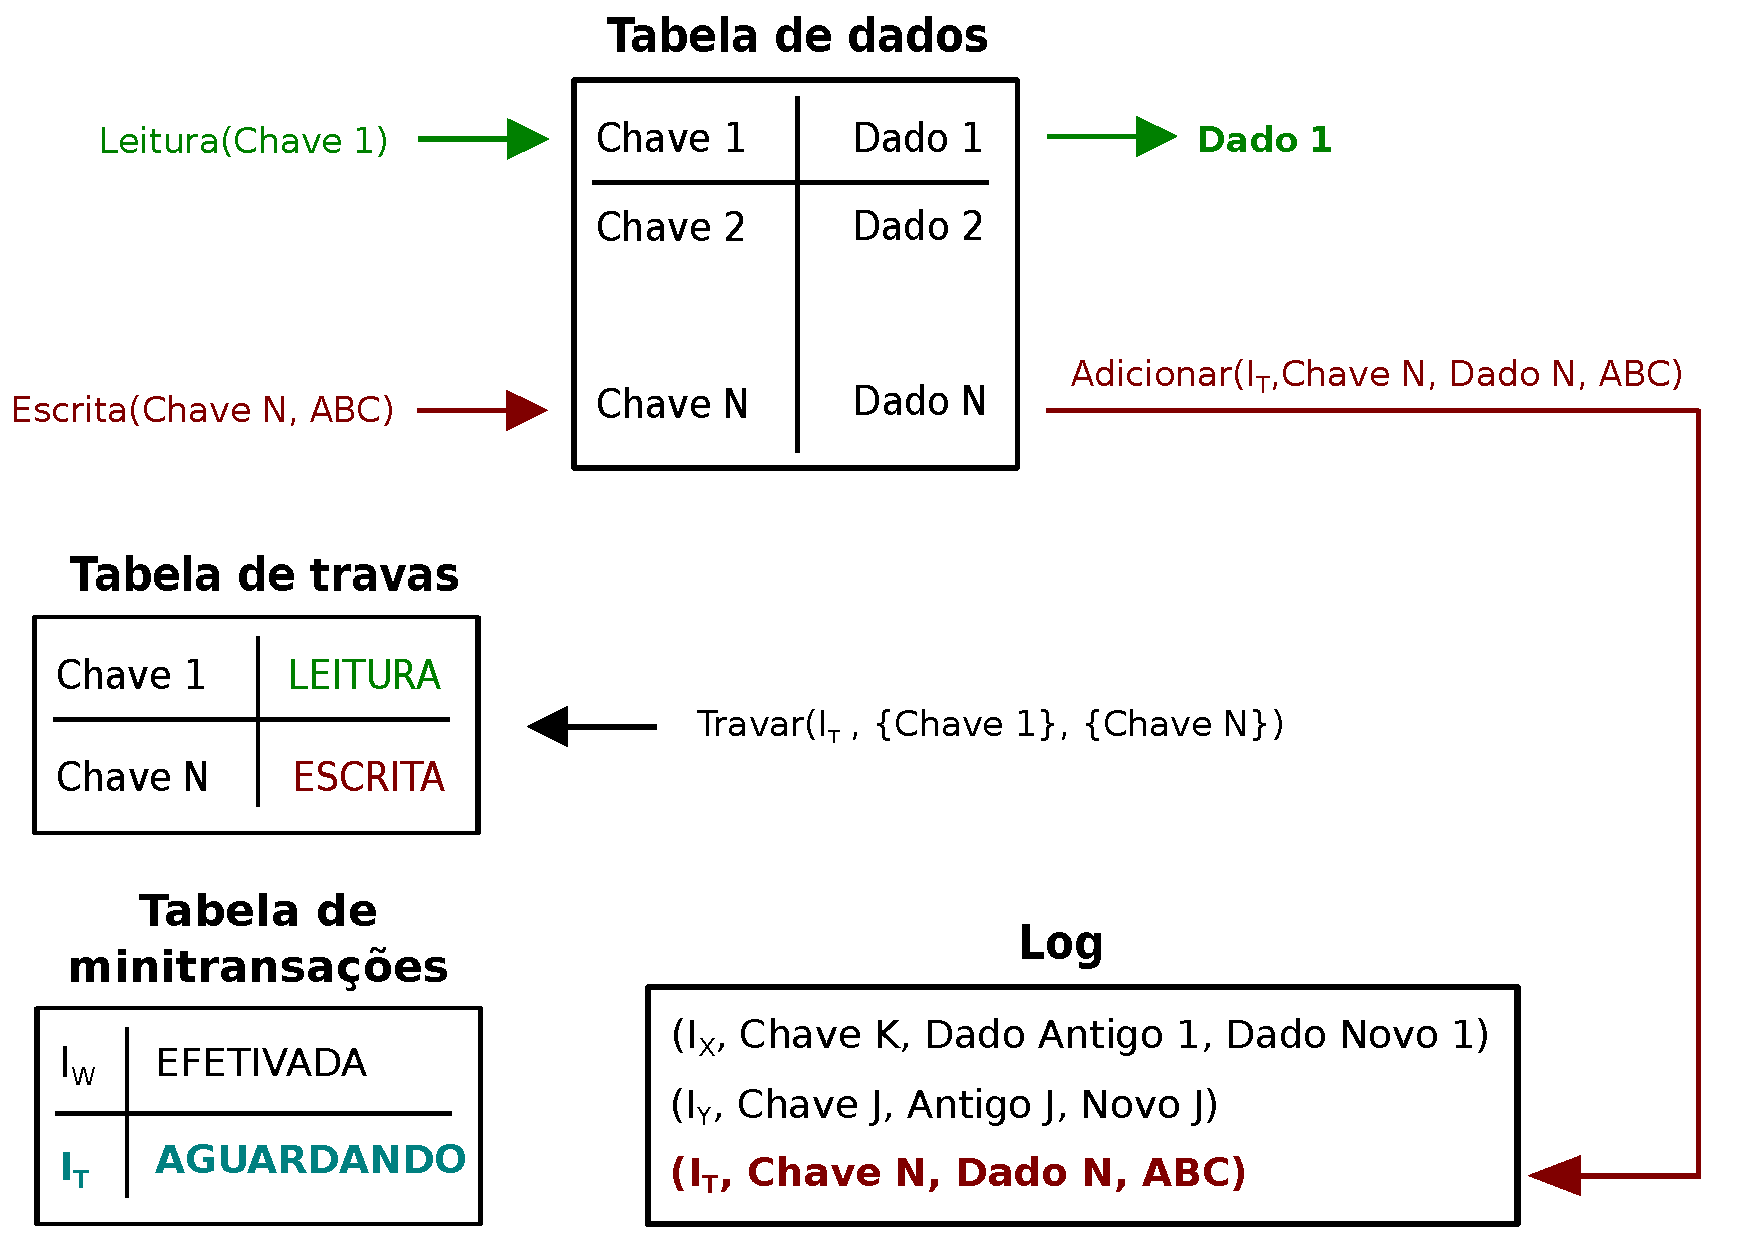
\includegraphics[width=.90\textwidth]{estruturas} 
  \caption{Operações sobre as estruturas e a relação entre elas}
  \label{fig:estruturas} 
\end{figure}

O comportamento do coordenador é descrito pelo Algoritmo \ref{alg:mini_coordenador}. $I_t$ é o identificador da transação, e é unicamente determinado pelo coordenador, relacionado com o identificador $I$ enviado pelo cliente. $C$ é o conjunto de comandos de extensão --- esses comandos indicarão ao nó de memória se a minitransação pode ser efetivada ou não, de forma análoga à operação de comparaçao das minitransações originais. $L$ é o conjunto de itens a serem lidos e $E$ é o conjunto de dados a serem atualizados ou inseridos. $L_j, Id[C_j]\text{ e } Id[E_j]$ são os conjuntos de identificadores da transação que estão armazenados em $P_j$, onde $L_j\text{ e }Id[C_J] \in D_j\text{ e }Id[E_j] \supseteq D_j$. $Op(c)$ indica a operação associada ao comando $c \in C_j$ e $Parametros(c)$ representa a lista de parâmetros de $c$. Cada participante $p_j$ mantém um \emph{log} de operações $log_{p_j}$, uma tabela de minitransações $mt_{p_j}$ e uma tabela de travas $travas_{p_j}$.

\begin{algorithm}
    \caption{Coordenador - recebe uma transação no formato $(I, C, L, E)$}
    \label{alg:mini_coordenador}
    \dontprintsemicolon
    \Inicio
    {    
        $repetir \gets false$\;
        \Repita{$repetir = false$}
        {
            $I_t \gets GerarIdentificador(I)$\;
            \ParaTodo{$p_j \in Participantes(C, L, E)$}
            {
                $Enviar(p_j, (I_t, C_j, L_j, E_j))$\;
            }
            $d \gets EFETIVAR$\;
            $R \gets \{\}$\;
            \ParaTodo{$p_j \in Participantes$}
            {
                $(v_j, r_j) \gets Receber(p_j)$\;
                \uSe{$v_j = FALHOU\_AO\_TRAVAR$}
                {    
                    $repetir \gets true$\;
                    $d \gets ABORTAR$\;
                }
                \uSenaoSe{$v_j = ABORTAR$}
                {
                    $repetir \gets false$\;
                    $d \gets ABORTAR$\;
                    $P \gets$ Descrição do Problema\;
                }
                \Senao 
                {
                    $repetir \gets false$\;
                    $R \gets r_j \cup R$\;
                }
            }
            \ParaTodo{$p_j \in Participantes$}
            {
                $Enviar(p_j, (d, I_t))$\;
            }
        }
        \eSe{$d \neq ABORTAR$}
        {
            $Enviar(Cliente, (I, R))$\;
        }
        {
            $Enviar(Cliente, (I, P))$\;
        }
    }
\end{algorithm}

\begin{algorithm}
    \caption{Execução - $p_j$ recebe $(I_t, C_j, L_j, E_j)$ de $c$}
    \label{alg:mini_participante1}
    \dontprintsemicolon
    \Inicio
    {
        \uSe{$Travar(C_j \cup L_j, E_j) = FALHOU$}
        {
            $Enviar(c, (FALHOU\_AO\_TRAVAR))$\;
        }
        \uSenaoSe{$(I_t, CANCELADA) \in mt_{p_j}$}
        {
            $Enviar(c, (ABORTAR, $``Cancelado pelo gerenciador''$))$\;
        }
        \Senao
        {
            $mt_{p_j} \gets (I_t, AGUARDANDO) \cup mt_{p_j}$\;
            $d \gets EFETIVAR$\;
            \ParaTodo{$c \in C_j$}
            {
                \Se{$Executar(Op(c), Id(c), Parametros(c)) = Erro$}
                {
                    $d \gets ABORTAR$\;
                }
            }
            $R_l \gets \{\}$\;
            \Se{$d = EFETIVAR$}
            {
                \ParaTodo{$l \in L_j$}
                {
                    $R_l \gets Ler(Id(l)) \cup R_l$\;
                }
                
                \ParaTodo{$e \in E_j$}
                {
                    $Adicionar(log_{p_j}, I_t, (Id(e), Ler(Id(e)), Dado(e)) )$\;
                }

                $Gravar(log_{p_j})$\;
            }
            {
                $Liberar(I_t)$\;
            }
            $Enviar(c, (d, R_l))$\;
        }
    }
\end{algorithm}

\begin{algorithm}
    \caption{Confirmação - $p_j$ recebe $(d, I_t)$ de $c$}
    \label{alg:mini_participante2}
    \dontprintsemicolon
    \Inicio
    {
        \eSe{$d = EFETIVAR$}
        {    
            \ParaTodo{$(Id(X),Dado(X),Dado'(X)) \in Selecionar(log_{p_j}, I_t)$}
            {    
                $Escrever(Id(X), Dado'(X))$\;
            }
            $mt_{p_j} \gets (I_t, EFETIVADA) \cup mt_{p_j}$\;
        }
        {
            $mt_{p_j} \gets (I_t, CANCELADA) \cup mt_{p_j}$\;
        }
        $Adicionar(log_{p_j}, I_t, d)$\;
        $Gravar(log_{p_j})$\;
        $Liberar(I_t)$\;
    }
\end{algorithm}

Todos os nós de memória que participarão da transação são identificadas através do conjunto de identificadores dos dados dos conjuntos $C$, $L$ e $E$ da transação por meio da função $Participantes$. O algoritmo envia uma minitransação com identificador $I_t$ para cada participante. Ao receber a minitransação, cada nó de memória segue o procedimento descrito no Algoritmo \ref{alg:mini_participante1}, primeiro adicionando a nova minitransação no conjunto de minitransações. Depois o nó de memória tenta obter todas as travas para acessar os dados especificados na minitransação---essa estratégia é usada para evitar problemas de esperas cíclicas (\emph{deadlocks}) entre diferentes minitransações. Uma resposta especial, $FALHOU\_AO\_TRAVAR$ é enviada caso não tenha sido possível obter alguma trava. Se conseguiu obter todas as travas, o nó de memória vai executar os comandos de extensão, e se algum deles retornar $ERRO$, a minitransação será abortada.

Após a execução, os participantes respondem à primeira fase do protocolo para o coordenador, que analisa cada resposta para descobrir o resultado da transação. Caso uma das respostas seja $FALHOU\_AO\_TRAVAR$, o coordenador deve abortar a transação em todos os participantes e iniciar novamente a execução. Uma resposta $ABORTAR$ indica que algum comando de extensão não foi bem sucedido, a transação é cancelada em todos os nós e o protocolo termina. Se todos os nós responderem com $EFETIVAR$, as respostas aos comandos de leitura são agregadas no conjunto $R$ e retornadas para a aplicação cliente. 

A decisão sobre a efetivação ou cancelamento da transação é comunicada a cada nó de memória, que segue o procedimento descrito no Algoritmo \ref{alg:mini_participante2}. Caso a decisão tenha sido para efetivar a minitransação, o participante irá vasculhar o seu \emph{log} por operações relacionadas à transação $I_t$ e irá executar essas transações, alterando a tabela de dados caso operações de escrita tenham sido especificadas na minitransação. A decisão sobre a efetivação ou cancelamento da minitransação é registrada no \emph{log} de cada participante e esse \emph{log} é gravado em disco.

Diferentemente do que ocorre no \emph{2PC}, o coordenador nunca escreve em um \emph{log}. Como os componentes de acesso estarão em geral nas mesmas máquinas que as aplicações cliente, e essas máquinas são consideradas menos confiáveis que as máquinas em que os nós de memória estarão, essa abordagem permite que a execução de uma minitransação possa continuar caso o coordenador fique indisponível. O procedimento para recuperação em casos de falhas nesse cenário é mais complexo do que o caso centralizado do 2PC, em que a recuperação de falhas é feita a partir do \emph{log} do coordenador.

A recuperação de falhas na nossa infraestrutura será efetuada pelo nó de gerenciamento. Esse procedimento pode ser ativado tanto manualmente quanto de forma automática. O nó de gerenciamento consulta os nós de memória sobre minitransações que estejam na situação $AGUARDANDO$ por mais que um determinado período de tempo e, caso haja alguma, o nó irá solicitar que essa minitransação seja abortada. Nesse caso, o participante irá mudar a situação da minitransação para $CANCELADA$, e o algoritmo \ref{alg:mini_participante1} irá validar essa situação (linha 4). Nos algoritmos descritos é assumido que a operação de união de conjuntos considerará a unicidade do elemento baseado no identificador da transação. Por exemplo, se o conjunto $mt_{p_j}$ já possuir um elemento $(k, S)$, sendo $k$ um identificador e $S$ uma situação, se tentarmos efetuar a operação $mt_{p_j} \cup (k, S_1)$, essa dupla irá substituir a dupla $(k,S)$ em $mt_{p_j}$.

O controle de concorrência efetuado pelos nós de memória visa oferecer uma forma de sequenciamento entre as operações de minitransações concorrentes que, de forma similar às transações sequencíaveis de bancos de dados convencionais \cite{vaca}, tem o efeito de garantir que as operações de uma minitransação não interfiram nas operações de outras minitransações. Para efetuar a leitura da chave $c$, o nó de memória deve primeiro tentar associar uma trava $LEITURA$ à chave $c$ na tabela de travas. Essa associação só pode ocorrer se não houver nenhuma trava do tipo $ESCRITA$ associada a essa chave. A associação de uma trava $ESCRITA$ só pode ocorrer se não houver nenhuma trava $LEITURA$ ou $ESCRITA$ associada à chave $c$. Este tipo de trava é chamada de trava leitor-escritor (\emph{read-write lock} \cite{ipc}), e permite que várias transações possam ler um determinado dado ao mesmo tempo mas somente uma pode escrever informações nesse dado, e somente se nenhuma outra transação estiver lendo ou escrevendo.

\section{Trabalhos relacionados}
\label{sec:trabalhos_relacionados}
O conceito de minitransações é introduzido como base para a construção de \emph{Sinfonia} \cite{sinfonia}, um sistema cujo foco é prover a base para o desenvolvimento de sistemas distribuídos de baixo nível, como sistemas de arquivos distribuídos, gerenciadores de travas ou serviços de comunicação de grupos de computadores, enquanto que o objetivo deste trabalho é utilizar as minitransações como base para a construção de uma infraestrutura que facilite o desenvolvimento de aplicações distribuídas de alto nível, como sistemas de comércio eletrônico ou redes sociais. 

\emph{Sinfonia} é composto também por nós de memória que armazenam os dados, mas a interface exposta por estes componentes é diferente: cada nó de memória mantém uma sequência de bytes puros, organizados em um espaço de endereçamento linear, sem nenhuma estrutura. Cada nó de memória possui um espaço de endereçamento separado de forma que os dados são referenciados por um par que especifica o nó de memória e o endereço deste dado. Em nossa infraestrutura, o acesso é feito através de uma única chave, que é um conjunto de bytes que faça sentido para a aplicação.

Ao invés de utilizar um coordenador separado como em nossa infraestrutura, \emph{Sinfonia} disponibiliza uma biblioteca que é compilada junto ao aplicativo cliente, e nesse caso o aplicativo cliente é o coordenador. Em nossa infraestrutura, o coordenador permite isolar a aplicação de detalhes da distribuição dos dados entre os nós de memória, e pode ser acessado pela rede. Acreditamos que esta abordagem seja mais efetiva que a abordagem que utiliza uma biblioteca, pois qualquer linguagem que permita a utilização da pilha TCP/IP poderá utilizar nossa infraestrutura, ao passo que se disponibilizarmos uma biblioteca, somente as linguagens para as quais uma biblioteca for escrita poderão usufruir da infraestrutra.

\cite{padilha} apresenta um sistema de armazenamento baseado em minitransações tolerante a falhas bizantinas. Em sistemas que toleram somente componentes com falhas simples (\emph{fail-stop components}), é assumido que um componente pode estar em dois estados: ativo e inativo. Se estiver em um estado ativo, o componente se comportará de acordo com a especificação do sistema. Se estiver inativo, o componente simplesmente para de interagir com o sistema. Essa é uma maneira simples e um tanto simplificada de lidar com falhas no sistema, mas é a forma utilizada por diversos sistemas, entre ele \emph{Sinfonia} e a nossa infraestrutura. A maneira mais geral de lidar com falhas é através de falhas bizantinas (\cite{byzantine}). Em sistemas que lidam com esse tipo de falha, um componente ativo pode se comportar de forma incorreta, enviando mensagens com conteúdo aleatório (correto ou incorreto), ou não enviando mensagem nenhuma. O tratamento de falhas bizantinas não será discutido neste trabalho.

Como nosso sistema, gerenciadores de bancos de dados relacionais também permitem a execução de transações, como Oracle e MySQL. O tipo de transação oferecida por esses sistemas é normalmente chamada de ACID (Atomicidade, Consistência, Isolamento e Durabilidade) \cite{vaca}. Essas transações podem ser usadas em cenários nos quais não conseguimos utilizar as minitransações, sendo portanto muito mais gerais. Porém, devido às propriedades que devem garantir, o uso dessas transações não permite escalar o banco de dados para um grande número de máquinas, algo que as minitransações permitem.

Existem diversos sistemas que visam o armazenamento escalável de informações e a disponibilização de serviços para facilitar o desenvolvimento de sistemas distribuídos, visando em geral a utilização em aplicações de internet de larga escala. Entre eles, podemos citar Bigtable (\cite{bigtable}), Dynamo (\cite{dynamo}), ZooKeeper (\cite{zookeeper}), PNUTS (\cite{pnuts}), entre outros. 

Bigtable é o sistema de armazenamento distribuído do Google que oferece uma abstração de um mapa ordenado, multi-dimensional, esparço e distribuído. Dynamo, da Amazon, é um sistema de armazenamento chave-valor que visa oferecer alta disponibilidade à aplicações. Esses dois sistemas permitem que dados sejam particionados e replicados para obter melhor performance e disponibilidade, mas permitem que diferentes máquinas possam ter versões diferentes de uma mesma informação. 

ZooKeeper é um sistema que provê serviços de coordenação e sincronização para a construção de sistemas distribuídos que utiliza o algoritmo Paxos (\cite{paxos}) para garantir consistência entre as operações. Como o foco do ZooKeeper é permitir a coordenação entre componentes de um sistema distribuído, sua capacidade de armazenamento é limitada (em um megabyte), e portanto não é utilizável como um repositório de dados.

PNUTS é o serviço de armazenamento de dados do Yahoo! que garante que todas as réplicas de um determinado dado armazenado executam as mesmas alterações, na mesma ordem. PNUTS permite a existência de várias versões de um dado, e oferece uma primitiva \emph{test-and-set-write}, que efetua uma escrita de dados somente se uma determinada versão do dado for encontrada, semelhante ao mecanismo das minitransações.

Por último, Hazelcast (\cite{hazelcast}) e Akka (\cite{akka}) são ferramentas para o desenvolvimento de sistemas distribuídos que visam eliminar a necessidade de comunicação explícita entre os participantes do sistema, oferecendo abstrações como estruturas de dados distribuídas ou memória transacional. Hazelcast oferece a programas rodando na \emph{JVM Java} implementações distribuídas das coleções da biblioteca padrão (\emph{Collection, Set, List e Map}). Akka permite a utilização de memória transacional por \emph{software} (\cite{stm}), uma abordagem que emprega o conceito de transação discutido neste trabalho em operações de leitura e escrita na memória principal do computador.

\chapter{Cronograma}
\label{chap:cronograma}
Os próximos passos no trabalho serão:

\begin{itemize}
\item Desenvolvimento da infraestrutura: deverão ser implementados os nós de memória, coordenador e gerenciador. Período: Julho/2012 - Janeiro/2013.
\item Desenvolvimento das aplicações de teste: aplicações simples que permitam explorar e analisar a utilização e a performance da infraestrutura. Período: Novembro/2012 - Março/2013.
\item Testes das aplicações: execução dos testes, coleta e análise dos dados obtidos. Período: Março/2013 - Julho/2013.
\end{itemize}

% cabeçalho para os apêndices
\renewcommand{\chaptermark}[1]{\markboth{\MakeUppercase{\appendixname\ \thechapter}} {\MakeUppercase{#1}} }
\fancyhead[RE,LO]{}
\appendix

% ---------------------------------------------------------------------------- %
\backmatter \singlespacing   % espaçamento simples
\bibliographystyle{alpha-ime}% citação bibliográfica alpha
\bibliography{bibliografia}  % associado ao arquivo: 'bibliografia.bib'

\end{document}